\documentclass[a4paper,11pt,twocolumn]{article}

\usepackage{aas_macros}

\usepackage[utf8]{inputenc}
\usepackage[T1]{fontenc}
\usepackage{lmodern}
%\usepackage{times}
%\usepackage[margin=2cm]{geometry}
\usepackage[a4paper]{geometry}
\usepackage{amsmath}
\usepackage{mathtools}
\usepackage{graphicx}
\usepackage{multirow}
\usepackage{multicol}
\usepackage{blindtext}
\usepackage{hyperref}
\usepackage{float}

\usepackage{pgfplotstable}
\usepackage{booktabs}
% \pgfplotsset{compat=1.18}

\usepackage[authoryear]{natbib}

\graphicspath{ {./images/} }

\usepackage[czech]{babel}
\usepackage{graphicx}
\usepackage{amsmath}
\usepackage{xspace}
\usepackage{url}
\usepackage{siunitx}
\usepackage{indentfirst}
\usepackage{subcaption}
\usepackage{caption}
\usepackage{tabularx}
\usepackage{rotating}
\usepackage{tikz}
\usepackage[labelformat=parens,labelsep=quad,skip=3pt]{caption}

\usepackage{color}
\usepackage{listings}

\definecolor{codegreen}{rgb}{0,0.6,0}
\definecolor{codegray}{rgb}{0.5,0.5,0.5}
\definecolor{codepurple}{rgb}{0.58,0,0.82}
\definecolor{backcolour}{rgb}{0.95,0.95,0.92}

\lstdefinestyle{mystyle}{
    backgroundcolor=\color{backcolour},
    commentstyle=\color{codegreen},
    keywordstyle=\color{magenta},
    numberstyle=\tiny\color{codegray},
    stringstyle=\color{codepurple},
    basicstyle=\ttfamily\footnotesize\centering,
    breaklines=true,
    captionpos=b,
    numbers=left,
    numbersep=5pt,
    showspaces=false,
    showstringspaces=false,
    showtabs=false,
    tabsize=2
}

\lstset{style=mystyle}

%\widowpenalty 10000 \clubpenalty 10000 \displaywidowpenalty 10000
\setcounter{topnumber}{3}
\setcounter{bottomnumber}{3}
\setcounter{totalnumber}{6}
\renewcommand\topfraction{0.9}
\renewcommand\bottomfraction{0.9}
\renewcommand\textfraction{0.1}
\intextsep=8mm \textfloatsep=8mm

\renewcommand{\thesection}{\arabic{section}.}
\renewcommand{\thesubsection}{\thesection\arabic{subsection}.}
\makeatletter \def\@seccntformat#1{\csname the#1\endcsname\hspace{1ex}} \makeatother


\begin{document}
    \twocolumn[
    \noindent\hrulefill
    \begin{center}
        \bigskip
        \huge Periodová analýza
        \vspace{0.2cm}
        \par \large F4191: Praktikum z astronomie 2
        \par \large Artem Gorodilov
        \vspace{0.2cm}
        \par \large 23. ~ledna 2025
        \bigskip
    \end{center}
    \noindent\hrulefill
    \bigskip
    ]

    \vskip10pt

    \section{Abstrakt}
        V této práci jsem analyzoval světelné křivky šesti neznámých objektů a také světelnou křivku hvězdy Kepler-1063. Pro analýzu jsem sestrojil periodogramy pro frekvence $< 10 ~\text{cyklů/den}$ a určil čtyři signifikantní frekvence, z nichž jsem získal odpovídající periody charakterizující hypotetické rekurentní změny systému. 
        
        Výpočty byly provedeny pomocí skriptu v Pythonu (viz. \citet{github}).

    \section{Úvod}
        \subsection{Periodogram}
            Periodogram je nástroj používaný k analýze časových řad, například světelných křivek hvězd, za účelem identifikace periodických signálů. Princip jeho činnosti spočívá v transformaci časových dat na frekvenční doménu a měření síly variability při různých frekvencích.

            Matematicky je periodogram založen na Lomb-Scarglově metodě, která je zvláště vhodná pro nerovnoměrně vzorkované časové řady. Tato metoda odhaduje periodogram jako:
            
            \begin{equation*}
                \begin{aligned}
                    P(f) = \frac{1}{2\sigma^2} \Bigg[ 
                    &\frac{\left( \sum_{i} w_i (x_i - \bar{x}) \cos(2\pi f (t_i - \tau)) \right)^2}
                    {\sum_{i} w_i \cos^2(2\pi f (t_i - \tau))} \\
                    &+ 
                    \frac{\left( \sum_{i} w_i (x_i - \bar{x}) \sin(2\pi f (t_i - \tau)) \right)^2}
                    {\sum_{i} w_i \sin^2(2\pi f (t_i - \tau))} 
                    \Bigg],
                \end{aligned}
            \end{equation*}

            kde $f$ je frekvence, $x_i$ jsou hodnoty dat (např. jas hvězdy), $t_i$ jsou odpovídající časy, $\sigma^2$ je rozptyl dat, $\bar{x}$ je průměr dat a $\tau$  je korekce pro fázi.
                
            Výstupem periodogramu jsou frekvence, které odpovídají dominantním periodicím v datech, například rotačním periodám hvězd nebo oběžným periodám exoplanet. Hlavní vrcholy v periodogramu představují frekvence, na kterých je variabilita nejvýraznější. Výška těchto vrcholů udává sílu variability na dané frekvenci. Významné vrcholy mají hodnoty, které výrazně převyšují úroveň šumu, jež v periodogramu funguje jako základní hladina. Šum slouží k odlišení skutečných signálů od náhodných fluktuací v datech.

            SNR (Signal-to-Noise Ratio) je poměr mezi silou signálu a úrovní šumu. V kontextu periodogramu se SNR vypočítává jako poměr výšky vrcholu (síly signálu) k průměrné nebo mediánové úrovni šumu. Matematicky lze SNR vyjádřit jako:

            \begin{equation*}
                \text{SNR} = \frac{P_{\text{peak}}}{P_{\text{noise}}},
            \end{equation*}

            kde $P_{\text{peak}}$ je hodnota výkonu na dané frekvenci (vrchol periodogramu) a $P_{\text{noise}}$ je úroveň šumu. Vysoká hodnota SNR naznačuje, že detekovaný signál je silnější než šum, a tím pádem pravděpodobně skutečný.

            FAP (False Alarm Probability) je pravděpodobnost, že detekovaný vrchol v periodogramu vznikl náhodně, vlivem šumu, a nikoli jako důsledek skutečné periodické variability. Nižší hodnota FAP znamená vyšší důvěru ve skutečnost detekovaného signálu.

        \subsection{Prewhitening}
            Prewhitening je iterativní metoda používaná k izolaci a odstranění dominantních periodických signálů z časové řady. Proces začíná výpočtem Lomb-Scargleho periodogramu, který identifikuje nejvýznamnější frekvenci na základě spektrální sily. Tato frekvence je následně upřesněna pomocí gaussovské aproximace, která poskytuje její přesnou hodnotu a nejistotu.

            Po určení dominantní frekvence jsou data fázově složena podle odpovídající periody a je provedeno sinusoidní přizpůsobení. Výsledný fit se odečte od původní časové řady, čímž vzniká reziduální signál, který je dále analyzován v další iteraci. Tento postup se opakuje, dokud nejsou izolovány všechny signifikantní frekvence nebo dokud není dosažen určitý práh, například nízký SNR.

        \subsection{Window funkce}
            Window funkce je analytický nástroj používaný při zpracování časových řad, zejména v Fourierově analýze a při výpočtu periodogramů, k popisu vzorkovací charakteristiky dat. Její hlavní úlohou je kvantifikovat artefakty, které vznikají vlivem omezené délky a nepravidelného rozmístění časových pozorování.

            V kontextu Lomb-Scargleho periodogramu je window funkce určena výpočtem periodogramu časové řady, která obsahuje jednotkovou hodnotu amplitudy ve všech časových bodech. Tento periodogram poskytuje informaci o frekvenčních složkách, které jsou inherentně přítomné v samotném vzorkování dat, nikoli ve skutečném signálu. Výsledkem je spektrum, které ukazuje rozložení vedlejších laloků a interferenčních efektů, které mohou ovlivnit přesnost identifikace frekvencí.

    \section{Zpracování dat}
        \subsection{Data}
            Analyzoval jsem světelné křivky šesti neznámých objektů. Každá křivka byla pozorována v časovém intervalu přibližně $300 ~\text{d}$.

            Pro analýzu periodického chování objektu Kepler-1063 (KepID: 2985767) jsem zkombinoval světelné křivky z několika pozorování Keplerovy čtvrti. Každé z pozorování mělo expoziční dobu $1800 ~\text{s}$ (kadence: dlouhá). Data byla získána a sestavena pomocí knihovny \texttt{lightkurve} \footnote{\url{https://lightkurve.github.io/lightkurve/}}. Celková doba pozorování byla $1470.46  ~ \text{d}$.

        \subsection{Pipeline}
            Pomocí funkce \texttt{analyze\_light\_curve()} jsem vykreslil světelnou křivku a analyzoval ji, abych získal periodogram. Funkce bere jako parametry názvy souboru nebo objektu Kepler, maximální počet signifikantních frekvencí na výstupu a maximální frekvenci vybranou pro analýzu. V mém případě jsou hodnoty posledních dvou parametrů následující: 
            
            \begin{center}
                \texttt{max\_frequencies=4}, \texttt{max\_frequency=10}.
            \end{center}

            Skript poté provede prewhitening pomocí funkce \texttt{prewhiten\_lightcurve()}. Tato funkce cyklicky vyhledává signifikantní frekvence. Za tímto účelem projdou původní data LombScargleovým fitováním, po kterém získáme frekvence a jejich síly pro danou časovou konfiguraci a zbytkový tok. Skript poté vyhledá maxima na grafu čas-frekvence pomocí funkce \texttt{find\_peaks()} dostupné v knihovně \texttt{SciPy} \footnote{\url{https://scipy.org/}}, provede Gaussův fit jejich vrcholů na periodogram, provede sinusovy fit fázově složené světelné křivky pro nalezenou frekvenci a opraví zbytkový tok z fitovaných dat. To pokračuje, dokud funkce nenajde 4 signifikantní frekvence. Skript také vypočítá Window funkci pomocí funkce \texttt{window\_function()}, která se následně použije pro vizuální analýzu periodogramu, SNR pro každou z nalezených frekvencí a vypočítá hodnoty FAP. 
            
            K výpočtu veličin a jejich nejistot byla použita knihovna Uncertinties pro Python. Chyby byly rozšířeny o Studentův koeficient (2-Tail Confidence Level) s ohledem na stupně volnosti pro každou hodnotu, pro interval spolehlivosti 68.27\%.

    \section{Vysledky}
        \subsection{Původní soubory dat}
            Světelné křivky pro soubory dat 1, 2, 3, 4, 5 a 6 jsou zobrazeny na obrázcích (\ref{fig:1_lc}), (\ref{fig:2_lc}), (\ref{fig:3_lc}), (\ref{fig:4_lc}), (\ref{fig:5_lc}) a (\ref{fig:6_lc}) resp. 
            
            Jejich odpovídající periodogramy jsou znázorněny na obrázcích (\ref{fig:1_per}), (\ref{fig:2_per}), (\ref{fig:3_per}), (\ref{fig:4_per}), (\ref{fig:5_per}) a (\ref{fig:6_per}). 

            Fázově složené světelné křivky pro každou nalezenou signifikantní frekvenci odvozenou ze zbytkového toku jsou zobrazeny na obrázcích (\ref{fig:1_phase_folded}), (\ref{fig:2_phase_folded}), (\ref{fig:3_phase_folded}), (\ref{fig:4_phase_folded}), (\ref{fig:5_phase_folded}) a (\ref{fig:6_phase_folded}).

            Fázově složené světelné křivky s nalezenými signifikantními frekvencemi superponované na původní světelnou křivku jsou zobrazeny na obrázcích (\ref{fig:1_phase_folded_orig}), (\ref{fig:2_phase_folded_orig}), (\ref{fig:3_phase_folded_orig}), (\ref{fig:4_phase_folded_orig}), (\ref{fig:5_phase_folded_orig}) a (\ref{fig:6_phase_folded_orig}).
            
            Frekvence, periody, síla, SNR a FAP jsou uvedeny v tabulkách (\ref{tab:1}), (\ref{tab:2}), (\ref{tab:3}), (\ref{tab:4}), (\ref{tab:5}) a (\ref{tab:6}). 

            \begin{table}[htbp]
                \centering
                \vspace{-1em}
                \resizebox{\columnwidth}{!}{%
                    \pgfplotstabletypeset[
                        col sep=comma,
                        string type,
                        every head row/.style={before row=\toprule, after row=\midrule},
                        every last row/.style={after row=\bottomrule},
                        columns/frequency/.style={column name=Frequency [c/d]},
                        columns/period/.style={column name=Period [d]},
                        columns/amplitude/.style={column name=Amplitude},
                        columns/snr/.style={column name=SNR},
                        columns/fap/.style={column name=FAP},
                    ]{output/1.csv}
                }
                \caption{Vysledky analýzy pro dataset 1.dat.}
                \label{tab:1}
            \end{table}
            
            \begin{table}[htbp]
                \centering
                \vspace{-2em}
                \resizebox{\columnwidth}{!}{%
                    \pgfplotstabletypeset[
                        col sep=comma,
                        string type,
                        every head row/.style={before row=\toprule, after row=\midrule},
                        every last row/.style={after row=\bottomrule},
                        columns/frequency/.style={column name=Frequency [c/d]},
                        columns/period/.style={column name=Period [d]},
                        columns/amplitude/.style={column name=Amplitude},
                        columns/snr/.style={column name=SNR},
                        columns/fap/.style={column name=FAP},
                    ]{output/2.csv}
                }
                \caption{Vysledky analýzy pro dataset 2.dat.}
                \label{tab:2}
            \end{table}

            \begin{table}[htbp]
                \centering
                \vspace{-2em}
                \resizebox{\columnwidth}{!}{%
                    \pgfplotstabletypeset[
                        col sep=comma,
                        string type,
                        every head row/.style={before row=\toprule, after row=\midrule},
                        every last row/.style={after row=\bottomrule},
                        columns/frequency/.style={column name=Frequency [c/d]},
                        columns/period/.style={column name=Period [d]},
                        columns/amplitude/.style={column name=Amplitude},
                        columns/snr/.style={column name=SNR},
                        columns/fap/.style={column name=FAP},
                    ]{output/3.csv}
                }
                \caption{Vysledky analýzy pro dataset 3.dat.}
                \label{tab:3}
            \end{table}

            \begin{table}[htbp]
                \centering
                \vspace{-2em}
                \resizebox{\columnwidth}{!}{%
                    \pgfplotstabletypeset[
                        col sep=comma,
                        string type,
                        every head row/.style={before row=\toprule, after row=\midrule},
                        every last row/.style={after row=\bottomrule},
                        columns/frequency/.style={column name=Frequency [c/d]},
                        columns/period/.style={column name=Period [d]},
                        columns/amplitude/.style={column name=Amplitude},
                        columns/snr/.style={column name=SNR},
                        columns/fap/.style={column name=FAP},
                    ]{output/4.csv}
                }
                \caption{Vysledky analýzy pro dataset 4.dat.}
                \label{tab:4}
            \end{table}

            \begin{table}[htbp]
                \centering
                \vspace{-2em}
                \resizebox{\columnwidth}{!}{%
                    \pgfplotstabletypeset[
                        col sep=comma,
                        string type,
                        every head row/.style={before row=\toprule, after row=\midrule},
                        every last row/.style={after row=\bottomrule},
                        columns/frequency/.style={column name=Frequency [c/d]},
                        columns/period/.style={column name=Period [d]},
                        columns/amplitude/.style={column name=Amplitude},
                        columns/snr/.style={column name=SNR},
                        columns/fap/.style={column name=FAP},
                    ]{output/5.csv}
                }
                \caption{Vysledky analýzy pro dataset 5.dat.}
                \label{tab:5}
            \end{table}

            \begin{table}[htbp]
                \centering
                \vspace{-1em}
                \resizebox{\columnwidth}{!}{%
                    \pgfplotstabletypeset[
                        col sep=comma,
                        string type,
                        every head row/.style={before row=\toprule, after row=\midrule},
                        every last row/.style={after row=\bottomrule},
                        columns/frequency/.style={column name=Frequency [c/d]},
                        columns/period/.style={column name=Period [d]},
                        columns/amplitude/.style={column name=Amplitude},
                        columns/snr/.style={column name=SNR},
                        columns/fap/.style={column name=FAP},
                    ]{output/6.csv}
                }
                \caption{Vysledky analýzy pro dataset 6.dat.}
                \label{tab:6}
            \end{table}
        
        \newpage
        \subsection{Kepler-1063}
            Světelná křivka pro Kepler-1063 je zobrazena na obrázku (\ref{fig:kplr_ls}). 
            
            Odpovídající periodogram je znázorněn na obrázku (\ref{fig:kplr_per}). 

            Fazově složené světelné křivky pro každou nalezenou signifikantní frekvenci odvozenou ze zbytkového toku jsou zobrazeny na obrázku (\ref{fig:kplr_phase_folded}).

            Fažově složené světelné křivky s nalezenými signifikantními frekvencemi superponované na původní světelnou křivku jsou zobrazeny na obrázku (\ref{fig:kplr_phase_folded_orig}).
            
            Frekvence, periody, síla, SNR a FAP pro Kepler-1063 jsou uvedeny v tabulce (\ref{tab:kplr}).

            \begin{table}[htbp]
                \centering
                \resizebox{\columnwidth}{!}{%
                    \pgfplotstabletypeset[
                        col sep=comma,
                        string type,
                        every head row/.style={before row=\toprule, after row=\midrule},
                        every last row/.style={after row=\bottomrule},
                        columns/frequency/.style={column name=Frequency [c/d]},
                        columns/period/.style={column name=Period [d]},
                        columns/amplitude/.style={column name=Amplitude},
                        columns/snr/.style={column name=SNR},
                        columns/fap/.style={column name=FAP},
                    ]{output/Kepler-1063.csv}
                }
                \caption{Vysledky analýzy pro Kepler-1063.}
                \label{tab:kplr}
            \end{table}

            \begin{figure}
                \centering
                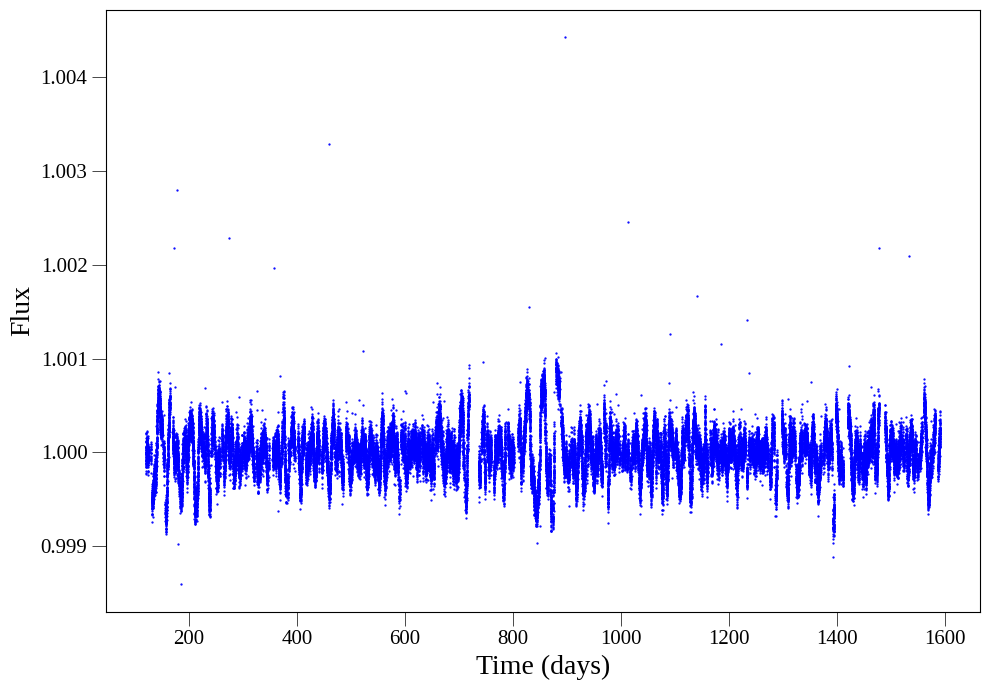
\includegraphics[width=0.5\textwidth]{lc/Kepler-1063_lc.png}
                \caption{Světelná křivka pro Kepler-1063.}
                \label{fig:kplr_ls}
            \end{figure}

    \section{Závěr}
        \subsection{Dataset 1}
            V souboru dat 1 jsou nejpravděpodobnější signifikantní frekvence $f_1 = 4.96799(3) ~\text{c/d}$ a $f_2 = 4.73131(1) ~\text{c/d}$ . Obě mají poměrně vysoký SNR a nízký FAP a nespadají do oblasti vrcholu Windowov funkce. Frekvence $f_3 = 1.10394(2) ~\text{c/d}$ má $\text{FAP} = 1$ a spadá do oblasti vrcholu Windowov funkce, což ji vylučuje ze seznamu pravděpodobných frekvencí. Frekvence $f_4 = 4.96742(2) ~\text{c/d}$ je blízká frekvenci $f_1 = 4.96799(3) ~\text{c/d}$, ale má mnohem menší FAP, což je také důvod k jejímu vyloučení ze seznamu pravděpodobných frekvencí.

            Při analýze fázově složených světelných křivek pro zbytkový tok je vidět, že fit každé frekvence kromě $f_4 = 4.96742(2) ~\text{c/d}$ je výrazná sinusoida. Analýza fázově složených světelných křivek získaných z původních dat ukazuje, že frekvence $f_3 = 1.10394(2) ~\text{c/d}$ zjevně není signifikantní frekvencí a lze ji vysvětlit mezerami v datech světelné křivky nebo jinou systematickou periodicitou nesouvisející s chováním objektu.

        \subsection{Dataset 2}
            V souboru dat 2 jsou nejpravděpodobnější signifikantní frekvence $f_1 = 3.04011(3) ~\text{c/d}$, $f_2 = 0.89276(7) ~\text{c/d}$ a $f_3 = 1.91776(1) ~\text{c/d}$. Obě mají poměrně vysoký SNR a nízký FAP, ale blíží se ploše vrcholu Windowov funkce. Frekvence $f_4 = 3.04152(3) ~\text{c/d}$ je blízká frekvenci $f_1 = 3.04011(3) ~\text{c/d}$, ale má mnohem nižší FAP, což je také důvodem k jejímu vyloučení z pravděpodobných frekvencí. 
            
            Při analýze fázově složených světelných křivek pro zbytkový tok vidíme, že fit každé frekvence kromě $f_4 = 3.04152(3) ~\text{c/d}$ je výrazná sinusoida. Analýza fázově složených světelných křivek získaných z původních dat ukazuje, že všechny frekvence nějakým způsobem odpovídají popisu periodicity objektu.

        \subsection{Dataset 3}
            V souboru dat 3 jsou nejpravděpodobnější signifikantní frekvence $f_1 = 2.35215(2) ~\text{c/d}$ a $f_2 = 3.50067(1) ~\text{c/d}$ . Obě mají poměrně vysoký SNR a nízký FAP a nespadají do oblasti vrcholu Windowov funkce. 
            Frekvence $f_3 = 2.92004(3) ~\text{c/d}$ je blízká frekvenci $f_1 = 2.35215(2) ~\text{c/d}$, ale má mnohem menší FAP a také spadá do oblasti vrcholů Windowov funkce, což je také důvodem k jejímu vyloučení ze seznamu pravděpodobných frekvencí. Frekvence $f_4 = 1.44576(5) ~\text{c/d}$ má $\text{FAP} = 1$ a spadá do oblasti vrcholu Windowov funkce, což ji vylučuje ze seznamu pravděpodobných frekvencí.
                
            Při analýze fázově složených světelných křivek pro zbytkový tok je vidět, že frekvence $f_1 = 2,35215(2) ~\text{c/d}$ a $f_2 = 3.50067(1) ~\text{c/d}$ vykazují výrazné sinusové chování. Frekvence $f_3 = 2.92004(3) ~\text{c/d}$ a $f_4 = 1.44576(5) ~\text{c/d}$ takové chování nevykazují. Analýza fázově složených světelných křivek získaných z původních dat ukazuje, že frekvence $f_4 = 1.44576(5) ~\text{c/d}$ zjevně není signifikantní frekvencí.

        \subsection{Dataset 4}
            V souboru dat jsou 4 nejpravděpodobnější signifikantní frekvence: $f_1 = 1.83302(2) ~\text{c/d}$ a $f_2 = 3.92680(2) ~\text{c/d}$ . Obě mají poměrně vysoký SNR a nízký FAP a nespadají do oblasti vrcholu Windowov funkce. Frekvence $f_3 = 6.04377(4) ~\text{c/d}$ má $\text{FAP} = 0.95$ a spadá do oblasti vrcholu Windowov funkce, což je také důvodem k jejímu vyloučení z pravděpodobných frekvencí. Frekvence $f_4 = 0.74150(2) ~\text{c/d}$ má $\text{FAP} = 1$ a spadá do oblasti vrcholu Windowov funkce, což ji vylučuje ze seznamu pravděpodobných frekvencí. 
                
            Při analýze fázově složených světelných křivek pro zbytkový tok je vidět, že frekvence $f_1 = 1.83302(2) ~\text{c/d}$ a $f_2 = 3.92680(2) ~\text{c/d}$ vykazují výrazné sinusové chování. Frekvence $f_3 = 6.04377(4) ~\text{c/d}$ a $f_4 = 0.74150(2) ~\text{c/d}$ takové chování nevykazují. Analýza fázově složených světelných křivek získaných z původních dat ukazuje, že frekvence $f_3 = 6.04377(4) ~\text{c/d}$ a $f_4 = 0.74150(2) ~\text{c/d}$ zjevně nejsou významné frekvence.

        \subsection{Dataset 5}
            V souboru dat 5 jsou všechny nalezené frekvence $f_1 = 7.62956(2) ~\text{c/d}$, $f_2 = 9.13811(2) ~\text{c/d}$, $f_3 = 7.83772(2) ~\text{c/d}$ a $f_4 = 2.16349(2) ~\text{c/d}$ pravděpodobné. Všechny mají vysoký SNR a nízký FAP a jsou mimo vrcholy okenní funkce.
                
            Při analýze fázově složených světelných křivek pro zbytkový tok je vidět, že fit pro všechny frekvence vykazuje výrazné sinusové chování. Analýza fázově složených světelných křivek získaných z původních dat rovněž ukazuje, že frekvence jsou vhodné pro vysvětlení periodického chování objektu.

        \subsection{Dataset 6}
            V souboru dat 6 jsou nejpravděpodobnější signifikantní frekvence $f_1 = 1.75607(4) ~\text{c/d}$, $f_2 = 1.88514(2) ~\text{c/d}$ a $f_3 = 4.55604(1) ~\text{c/d}$. Obě mají poměrně vysoký SNR a nízký FAP a nespadají do oblasti vrcholu Windowovy funkce. Frekvence $f_4 = 9.25930(8) ~\text{c/d}$ má $\text{SNR} = 15.3$ a $\text{FAP} = 0.31$.
    
            Analýza fázově složených světelných křivek pro zbytkový tok ukazuje, že fit každé frekvence kromě $f_4 = 9.25930(8) ~\text{c/d}$ je výrazná sinusoida. Analýza fázově složených světelných křivek získaných z původních dat ukazuje, že frekvence $f_4 = 9.25930(8) ~\text{c/d}$ není významnou frekvencí.

        \subsection{Kepler-1063}
            Při analýze světelné křivky Keplera-1063 se ukázalo, že frekvence v každé iteraci prewhiteningové funkce konvergují k hodnotě okolo $f = 0.0367 ~\text{c/d}$, což odpovídá periodě $P = 27.24 ~\text{c/d}$. Avšak pro frekvenci $f_1 = 0.03670(2) ~\text{c/d}$ při vysokém SNR je hodnota $\text{FAP} = 1$. A pro ostatní frekvence nebyl výpočet FAP v zásadě proveden. 

            Fázově složené světelné křivky pro data získaná ze zbytkového toku ukazují, že poslední tři frekvence vykazují sinusové chování, zatímco první nikoli. Fázově složené světelné křivky pro původní data nevykazují v zásadě žádné sinusové chování. 
            
            To vše s vysokou pravděpodobností znamená, že mnou nalezená perioda není periodou popisující periodické chování objektu. Navíc víme, že Kepler-1063 má exoplanetu Kepler-1063b s periodou $\text{P} = 14.08 ~\text{d}$ (viz. \citet{holczer2016} a \citet{morton2016}) . Hned je vidět, že mnou nalezená perioda je téměř přesně poloviční než perioda, kterou má exoplaneta. Možná je to jen náhoda, nicméně se pokusím spekulovat, proč by tomu tak mohlo být. Je možné, že se překrývají dva tranzity s různou hloubkou. Největší vrchol ve spektru musí být harmonickou skutečné periody. Ve skutečnosti se zdá, že zde dochází k tomu, že oba tranzity jsou interpretovány jako výsledek stejného signálu, zatímco ve skutečnosti budou mít oba tranzity mírně odlišné hloubky a tvary.

            Fázově složená světelná křivka pro původní data s poloviční periodou $\text{P} = 13.62 ~\text{d}$ je znázorněna na obrázku \ref{fig:Kepler-1063_phase_folded_orig_teor}. Ani z ní nelze pozorovat sinusové chování. Problém možná spočívá v tom, že data mají určitý trend, který je třeba před analýzou vyloučit.

    % \newpage
    \bibliographystyle{abbrvnat}
    \bibliography{bibliography}
        
    %%%% Světelné křivky %%%%
    \begin{figure*}%[htbp]
        \centering
        \begin{subfigure}[t]{0.48\textwidth}
            \centering
            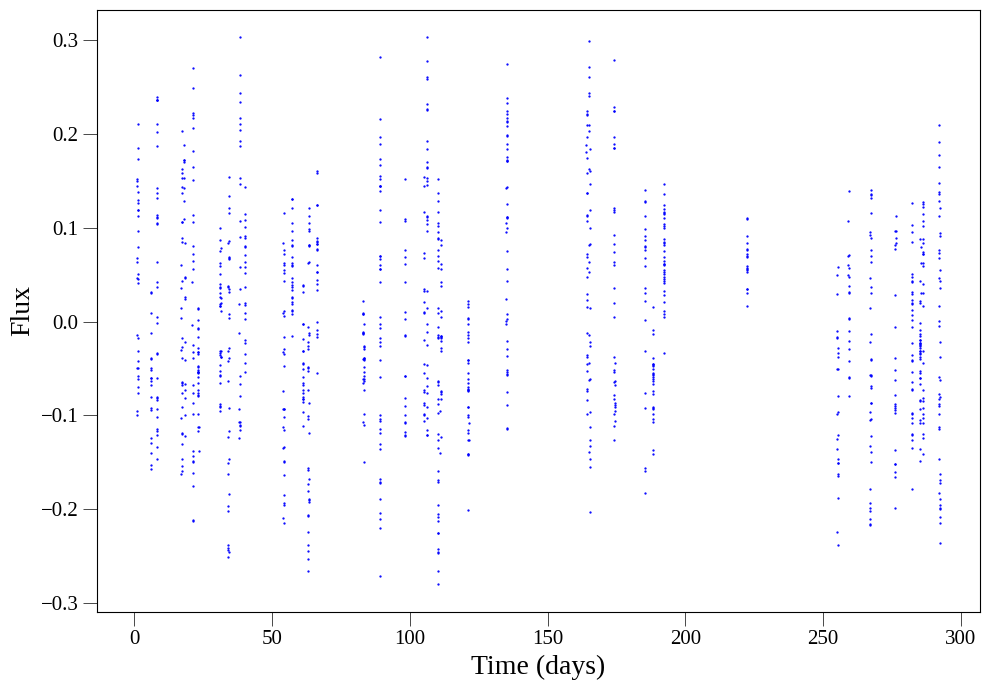
\includegraphics[width=\textwidth]{lc/1_lc.png}
            \caption{Světelná křivka pro dataset 1.dat.}
            \label{fig:1_lc}
        \end{subfigure}
        \hfill
        \begin{subfigure}[t]{0.48\textwidth}
            \centering
            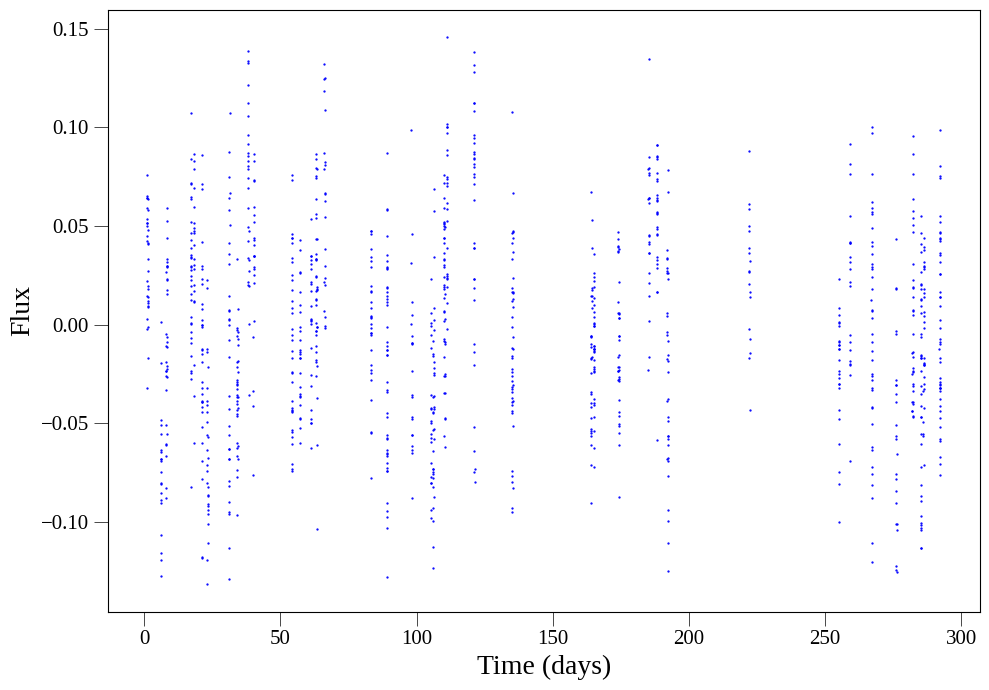
\includegraphics[width=\textwidth]{lc/2_lc.png}
            \caption{Světelná křivka pro dataset 2.dat.}
            \label{fig:2_lc}
        \end{subfigure}
        \hfill
        \begin{subfigure}[t]{0.48\textwidth}
            \centering
            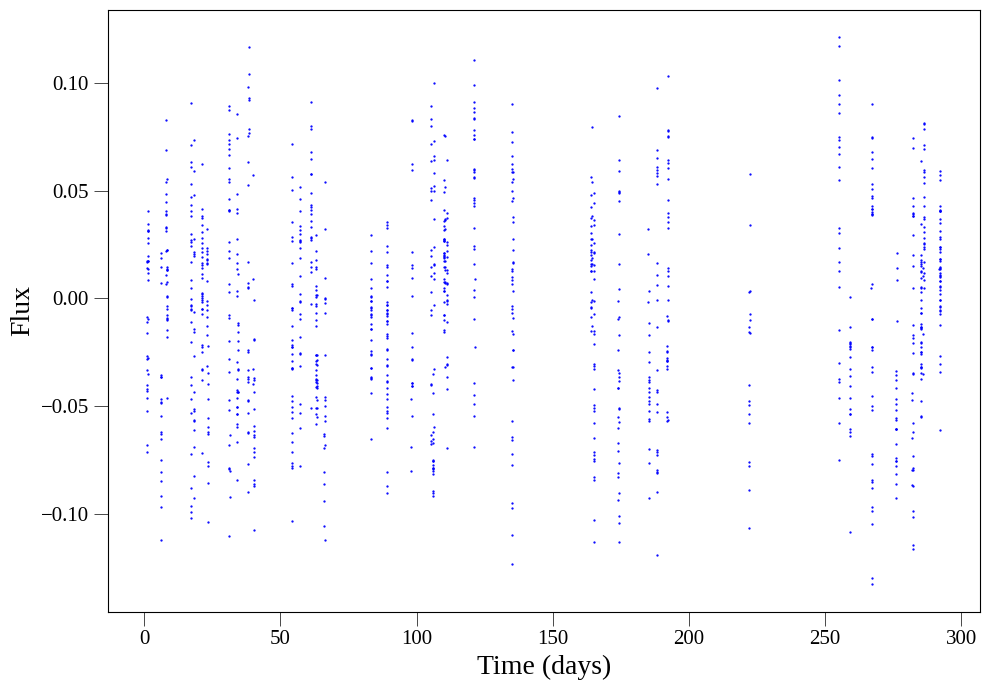
\includegraphics[width=\textwidth]{lc/3_lc.png}
            \caption{Světelná křivka pro dataset 3.dat.}
            \label{fig:3_lc}
        \end{subfigure}
        \vspace{10pt}
        \begin{subfigure}[t]{0.48\textwidth}
            \centering
            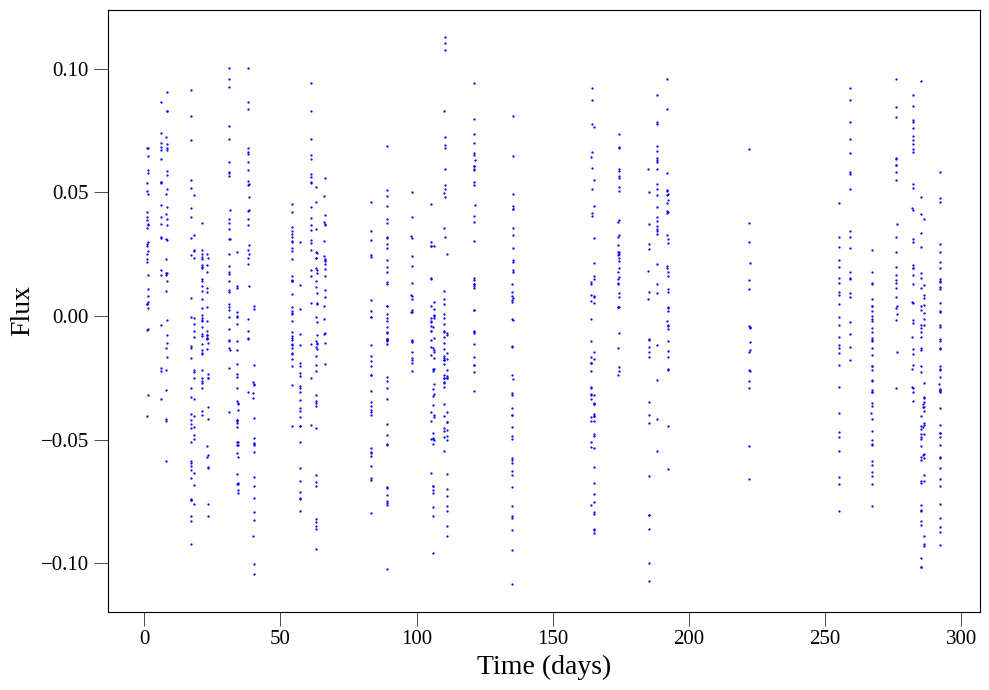
\includegraphics[width=\textwidth]{lc/4_lc.png}
            \caption{Světelná křivka pro dataset 4.dat.}
            \label{fig:4_lc}
        \end{subfigure}
        \hfill
        \begin{subfigure}[t]{0.48\textwidth}
            \centering
            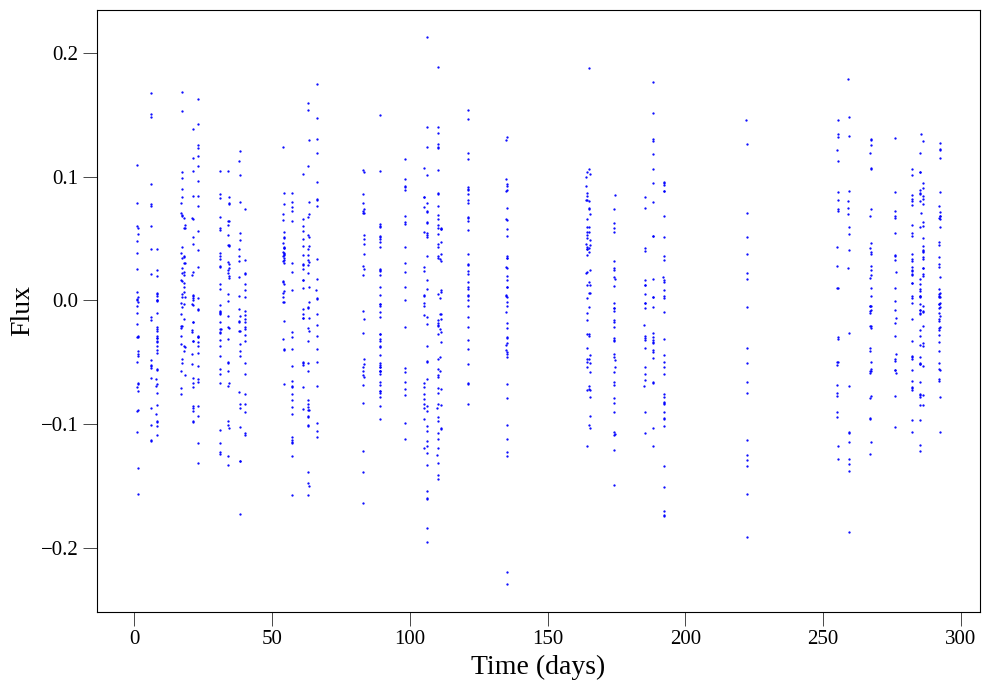
\includegraphics[width=\textwidth]{lc/5_lc.png}
            \caption{Světelná křivka pro dataset 5.dat.}
            \label{fig:5_lc}
        \end{subfigure}
        \hfill
        \begin{subfigure}[t]{0.48\textwidth}
            \centering
            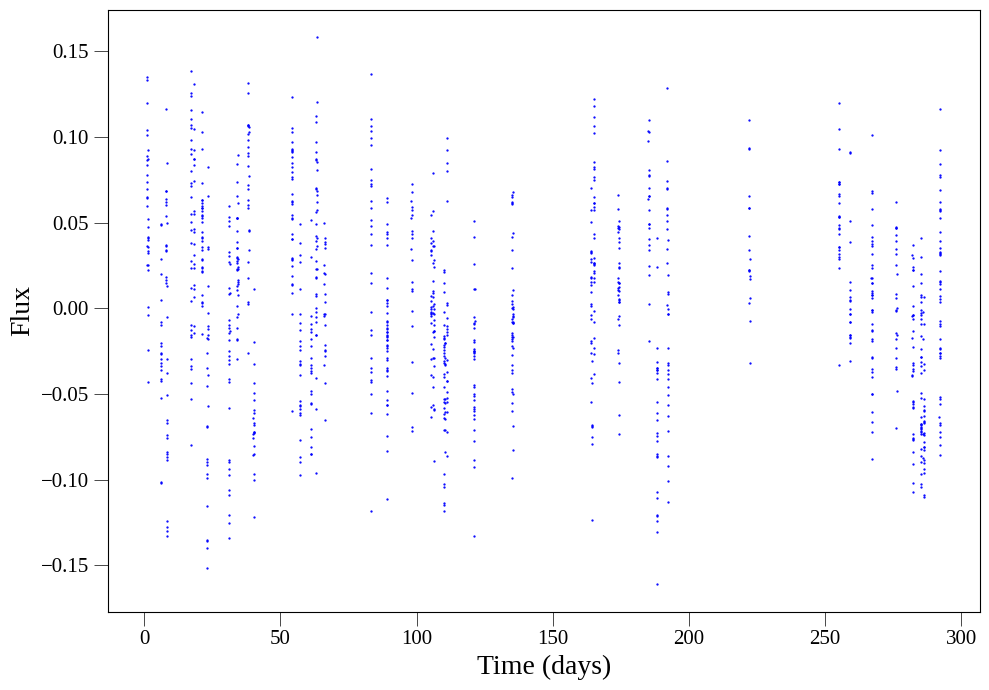
\includegraphics[width=\textwidth]{lc/6_lc.png}
            \caption{Světelná křivka pro dataset 6.dat.}
            \label{fig:6_lc}
        \end{subfigure}
        \caption{Světelné křivky pro všechny datasety.}
        \label{fig:all_lc}
    \end{figure*}

    %%%% Periodogramy %%%%
    \begin{figure*}
        \centering
        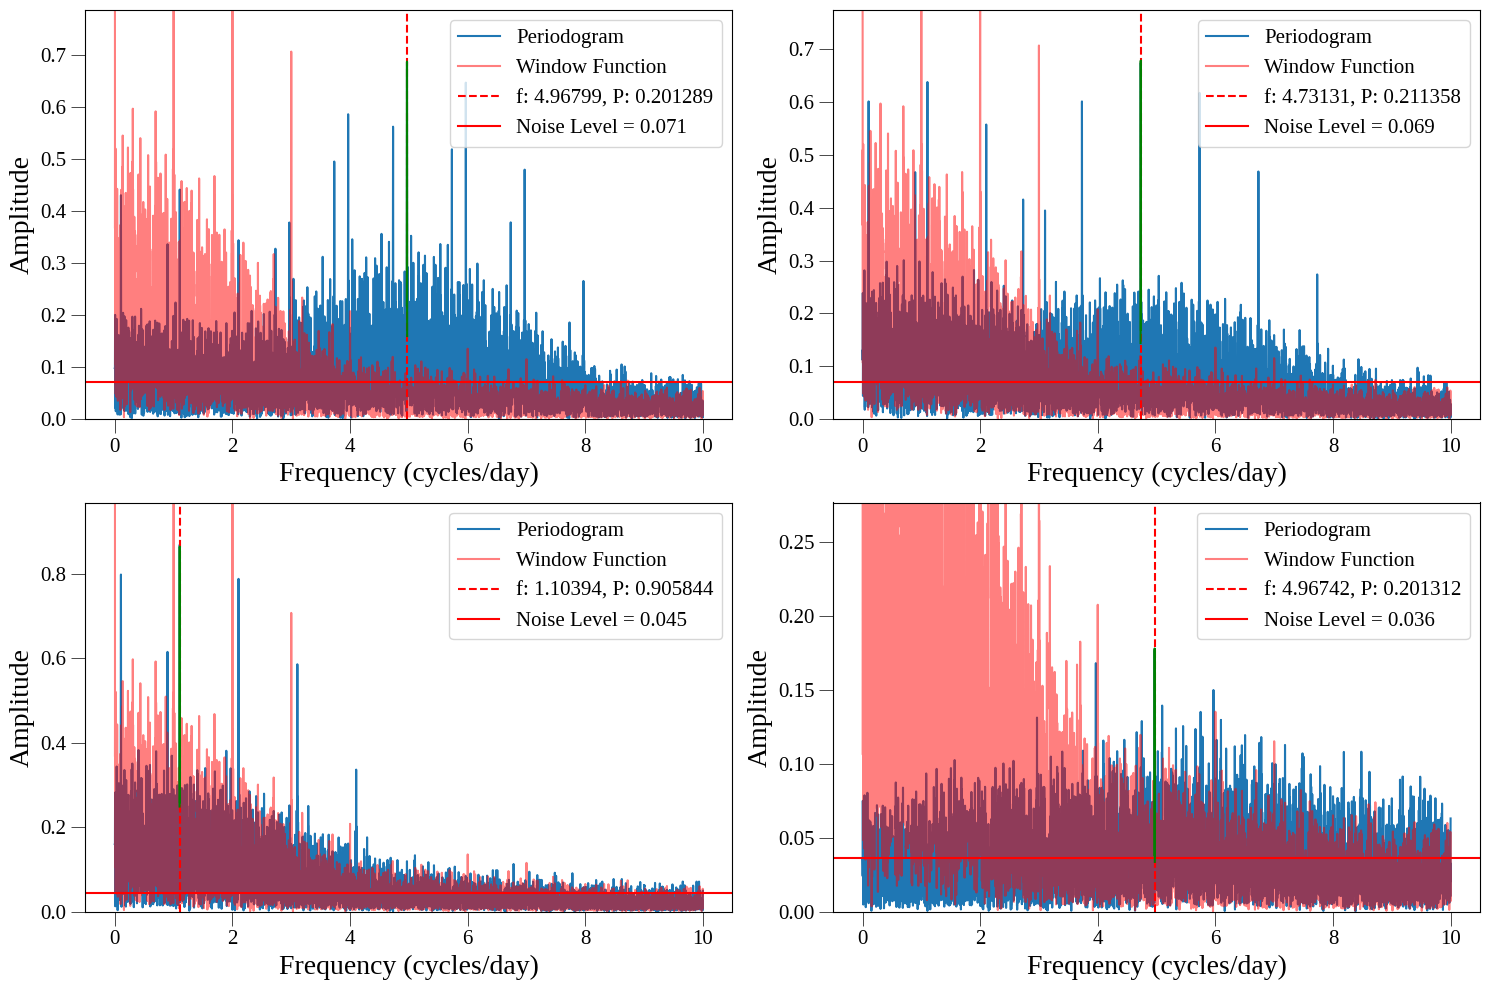
\includegraphics[width=0.9\textwidth]{period/1_per.png}
        \caption{Periodogram pro dataset 1.dat.}
        \label{fig:1_per}
    \end{figure*}

    \begin{figure*}
        \centering
        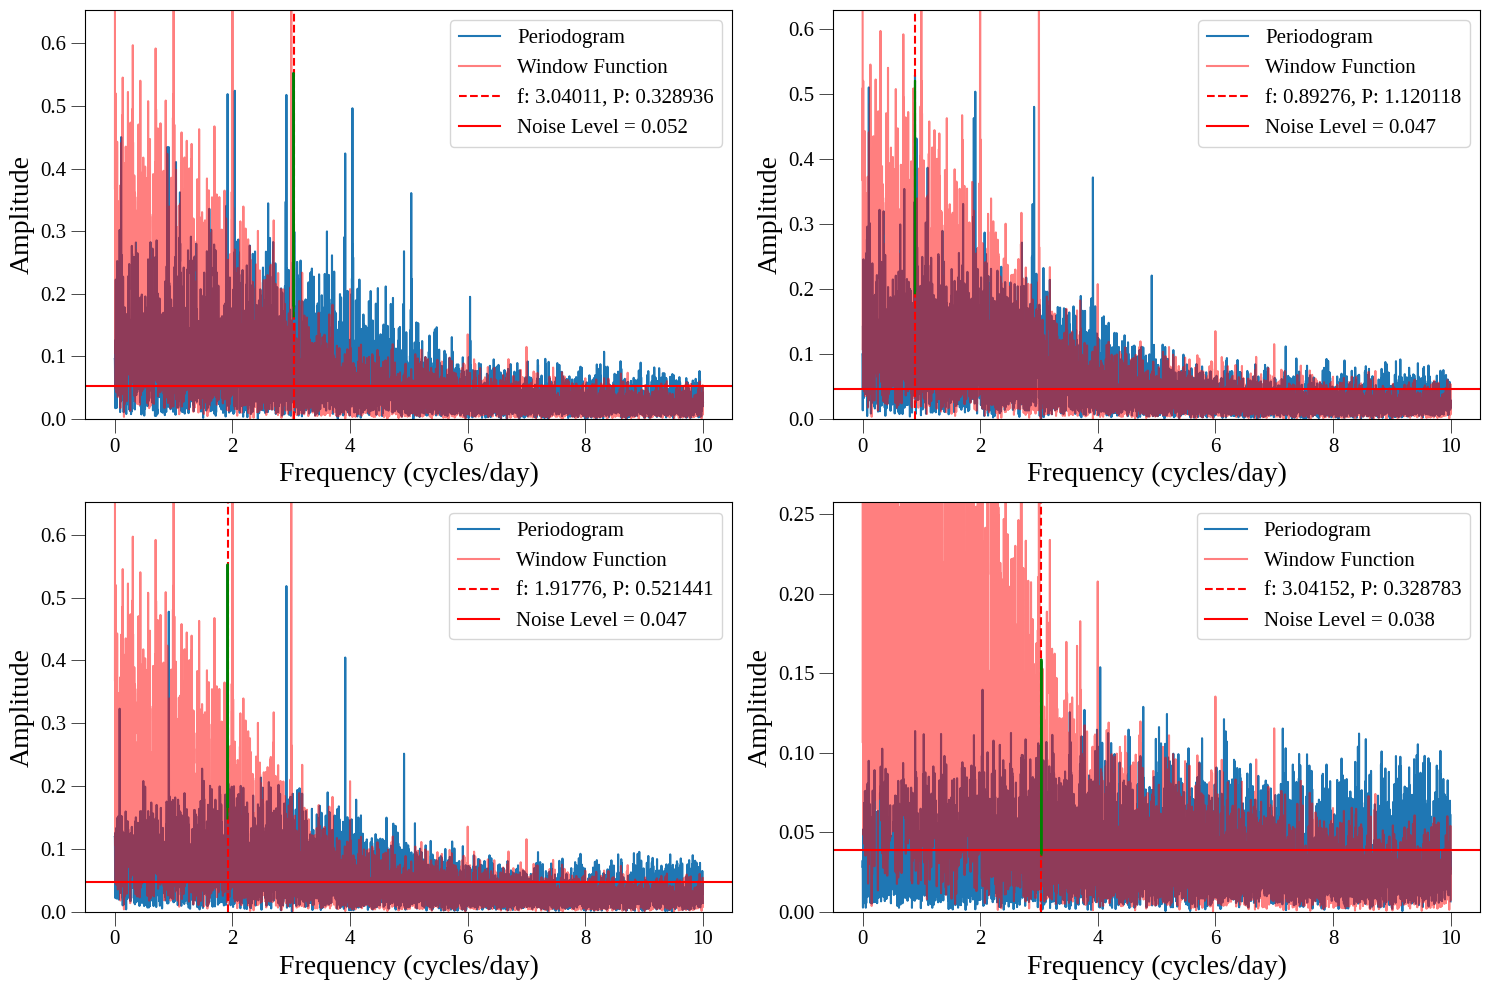
\includegraphics[width=0.9\textwidth]{period/2_per.png}
        \caption{Periodogram pro dataset 2.dat.}
        \label{fig:2_per}
    \end{figure*}

    \begin{figure*}
        \centering
        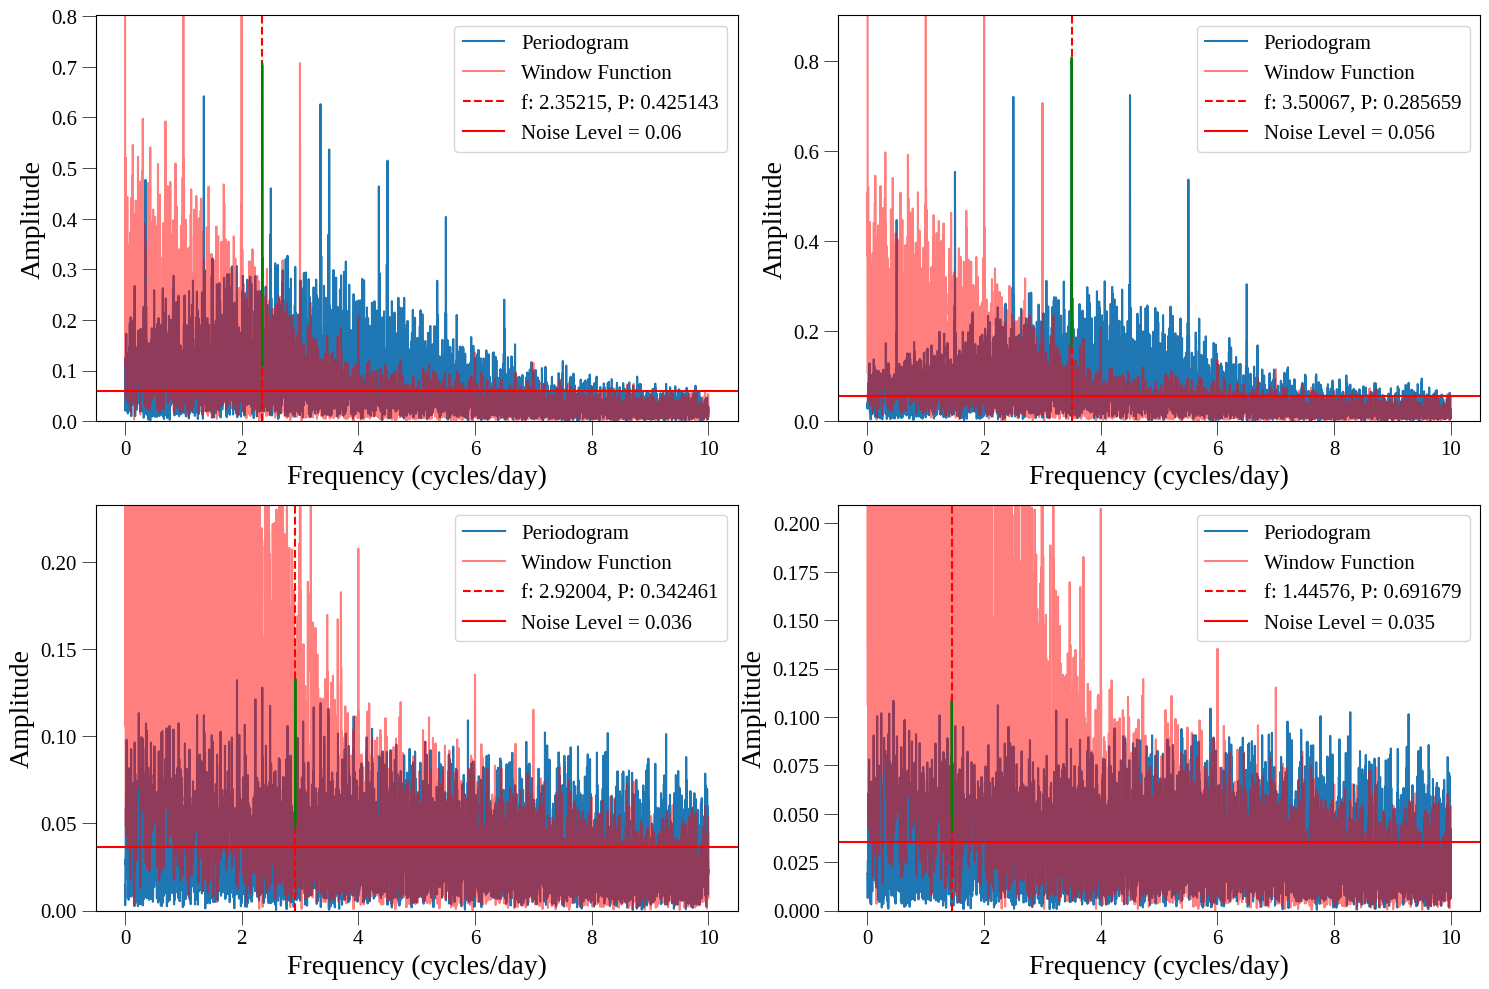
\includegraphics[width=0.9\textwidth]{period/3_per.png}
        \caption{Periodogram pro dataset 3.dat.}
        \label{fig:3_per}
    \end{figure*}

    \begin{figure*}
        \centering
        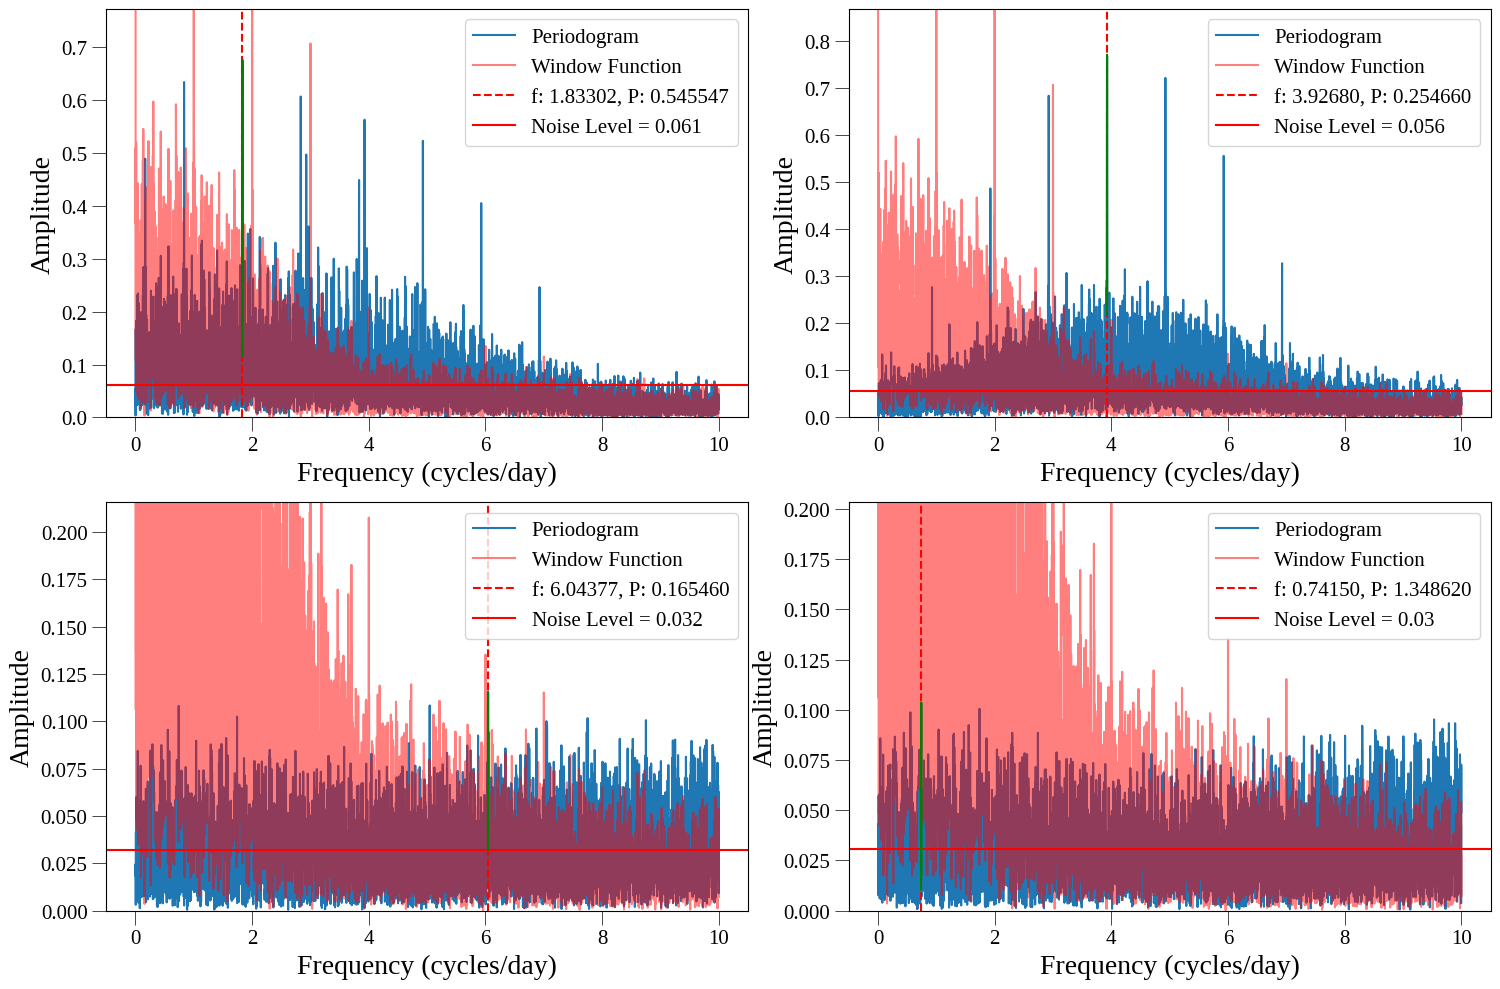
\includegraphics[width=0.9\textwidth]{period/4_per.png}
        \caption{Periodogram pro dataset 4.dat.}
        \label{fig:4_per}
    \end{figure*}

    \begin{figure*}
        \centering
        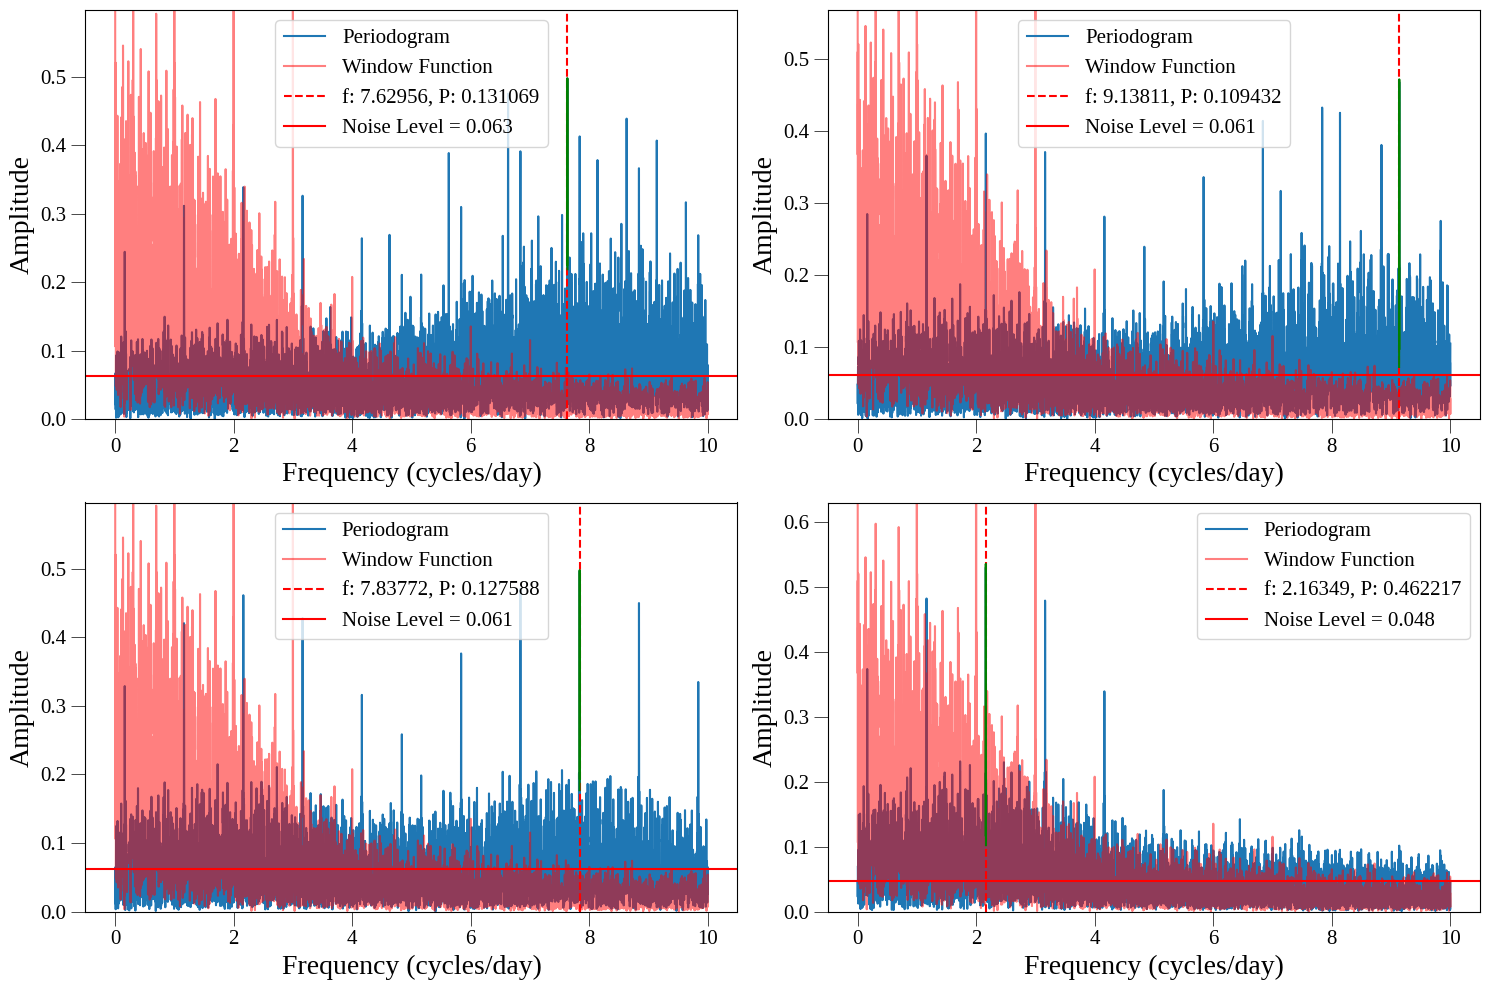
\includegraphics[width=0.9\textwidth]{period/5_per.png}
        \caption{Periodogram pro dataset 5.dat.}
        \label{fig:5_per}
    \end{figure*}

    \begin{figure*}
        \centering
        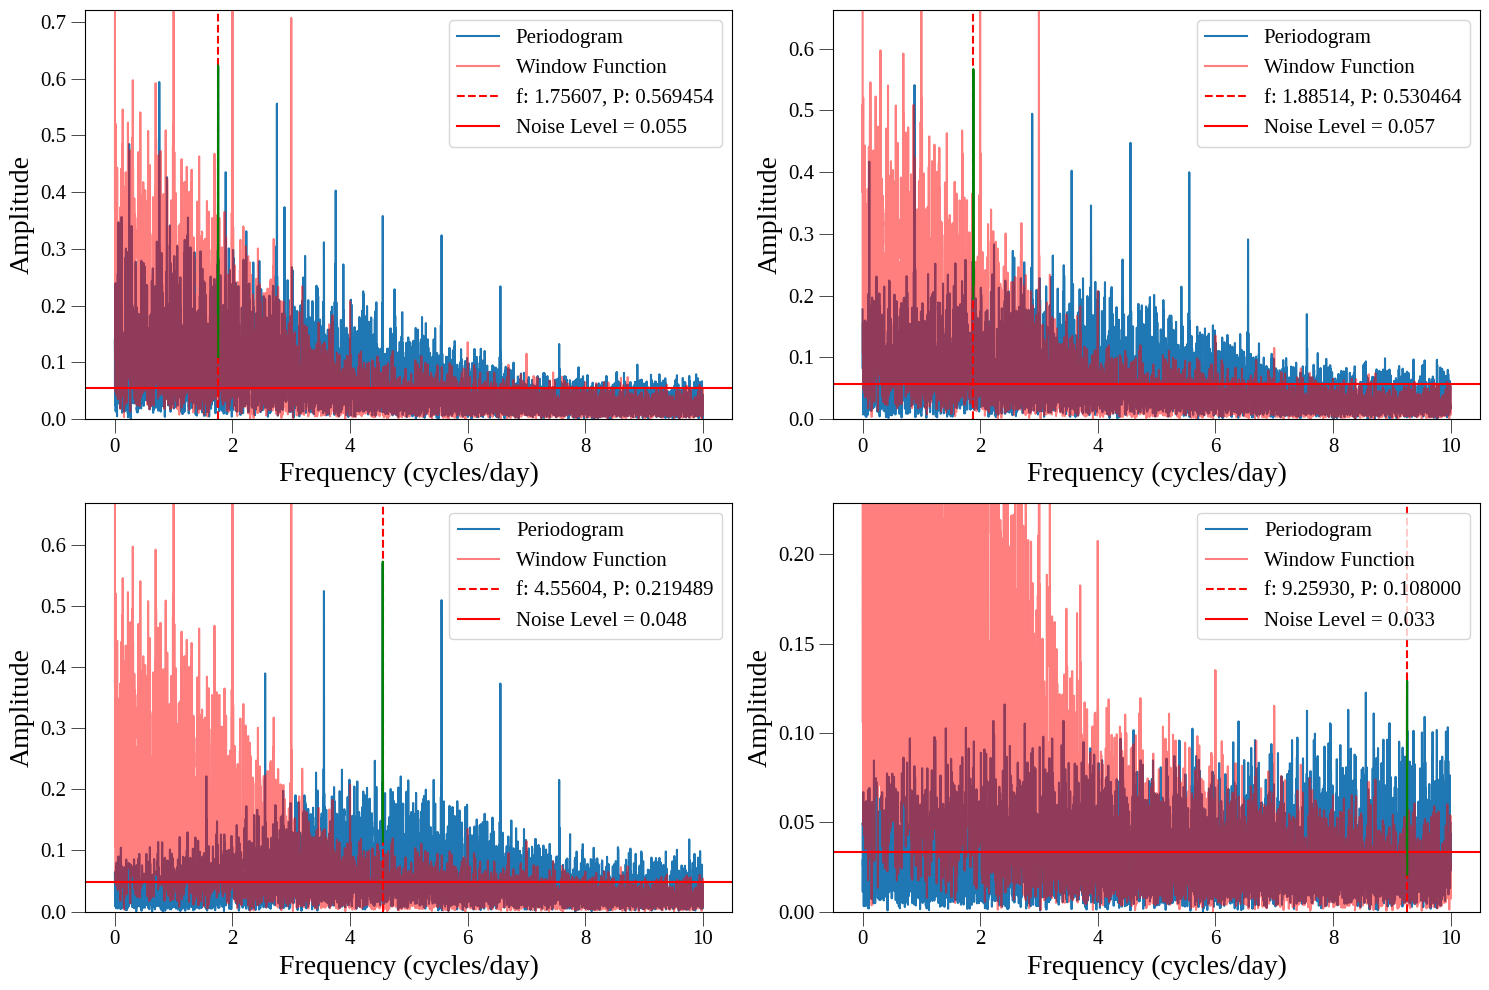
\includegraphics[width=0.9\textwidth]{period/6_per.png}
        \caption{Periodogram pro dataset 6.dat.}
        \label{fig:6_per}
    \end{figure*}

    %%%% Fázově složené světelné křivky %%%%
    \begin{figure*}
        \centering
        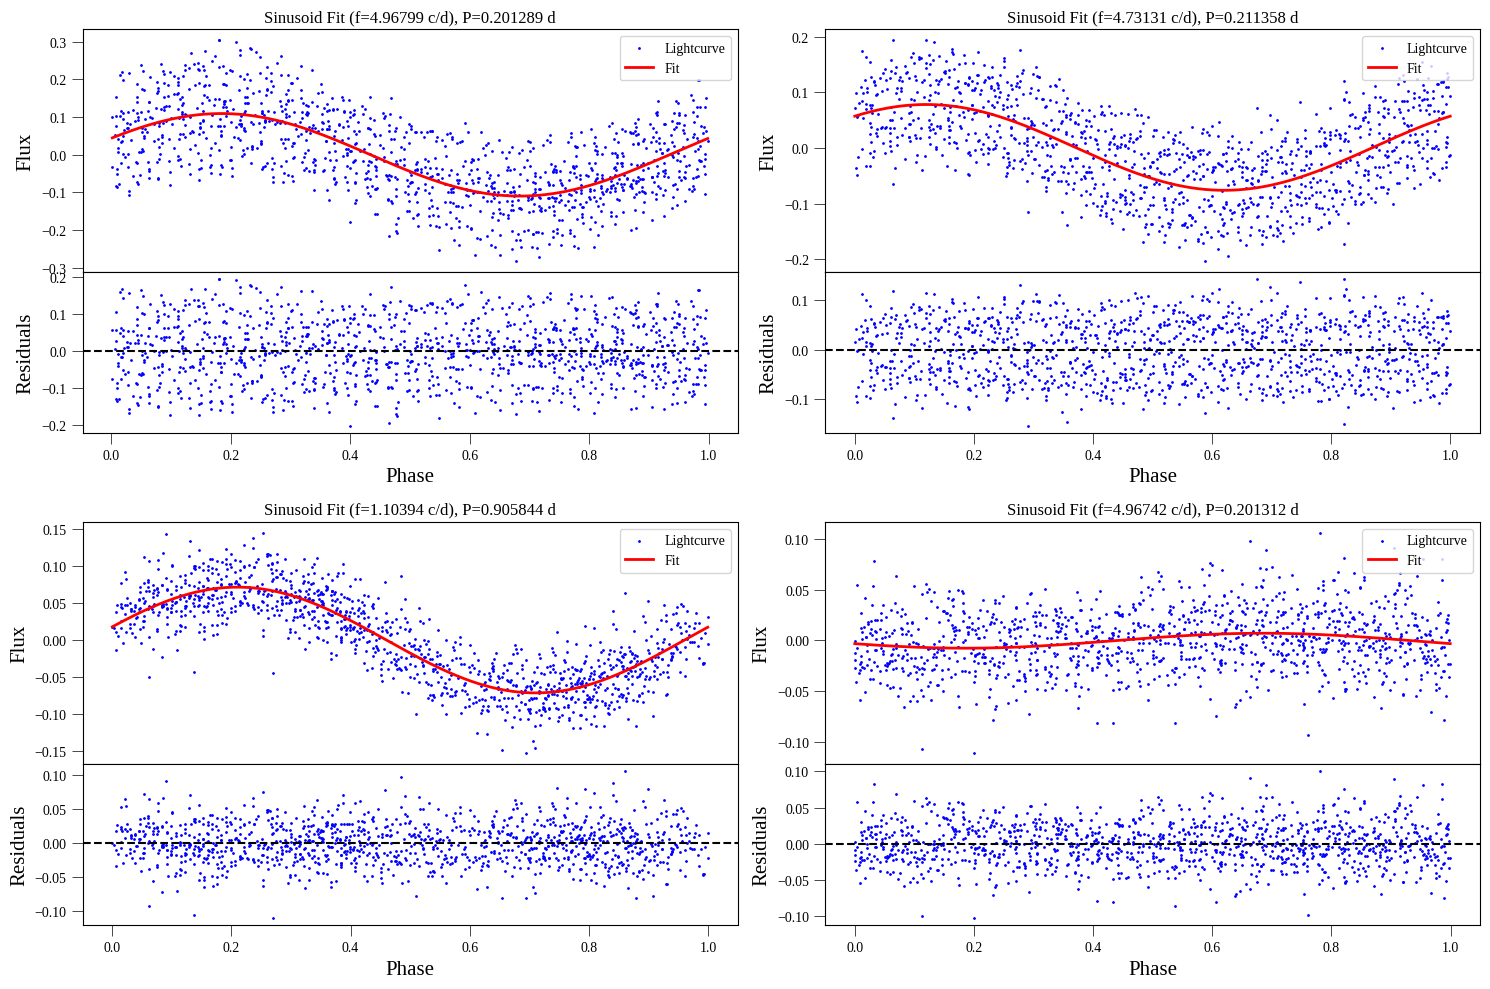
\includegraphics[width=0.9\textwidth]{phase/1_phase_folded.png}
        \caption{Fázově složená světelná křivka pro dataset 1.dat.}
        \label{fig:1_phase_folded}
    \end{figure*}

    \begin{figure*}
        \centering
        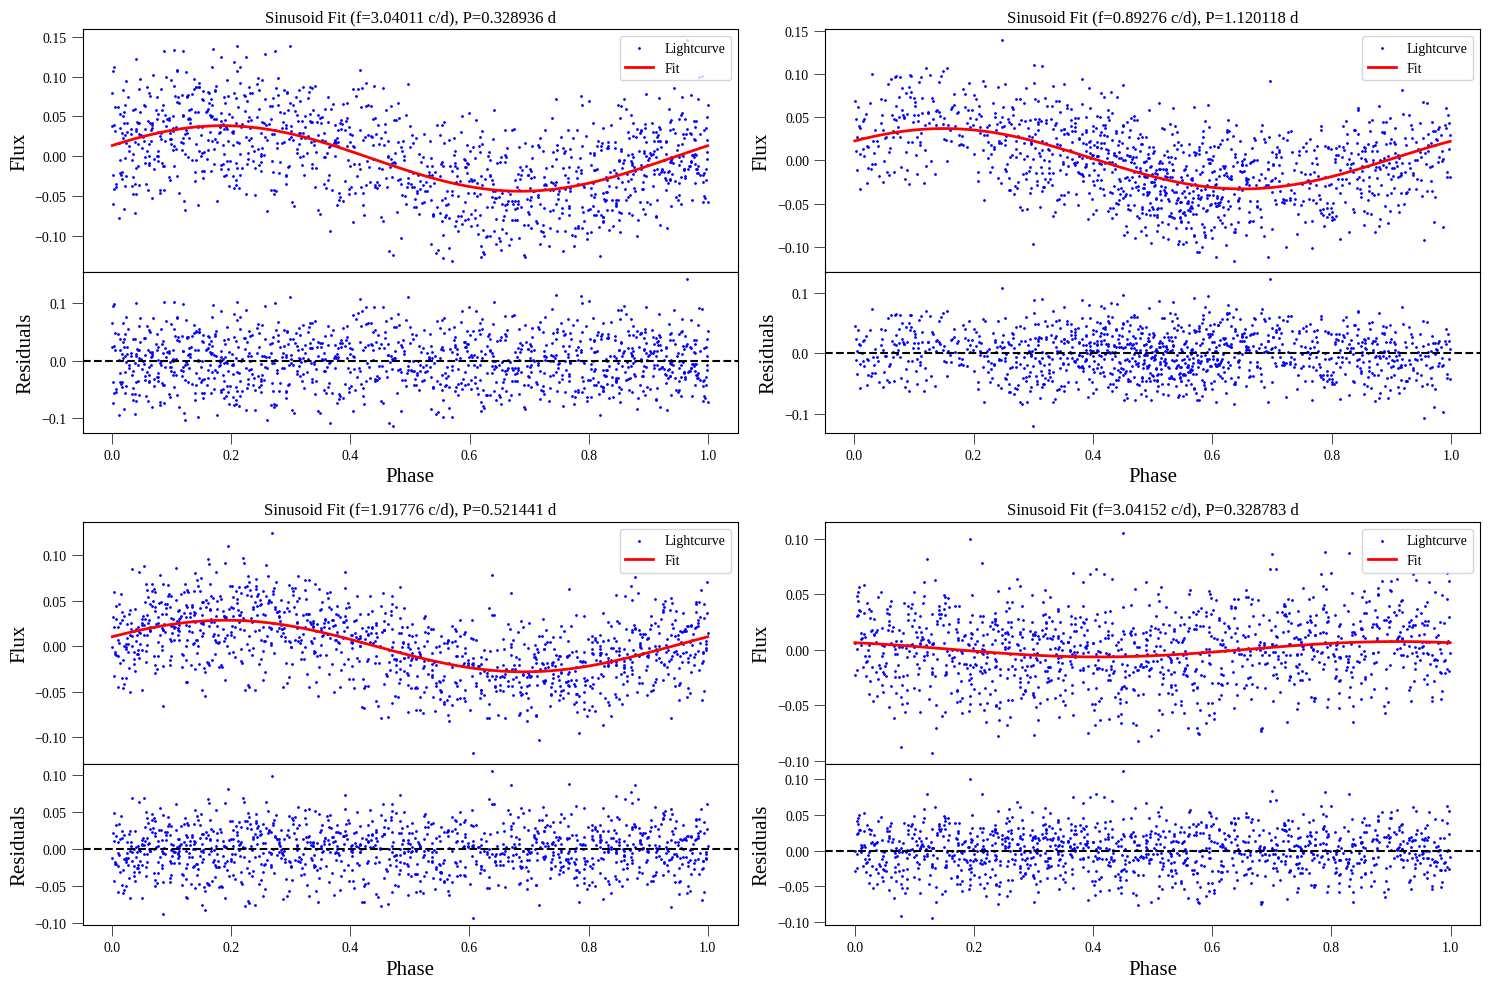
\includegraphics[width=0.9\textwidth]{phase/2_phase_folded.png}
        \caption{Fázově složená světelná křivka pro dataset 2.dat.}
        \label{fig:2_phase_folded}
    \end{figure*}

    \begin{figure*}
        \centering
        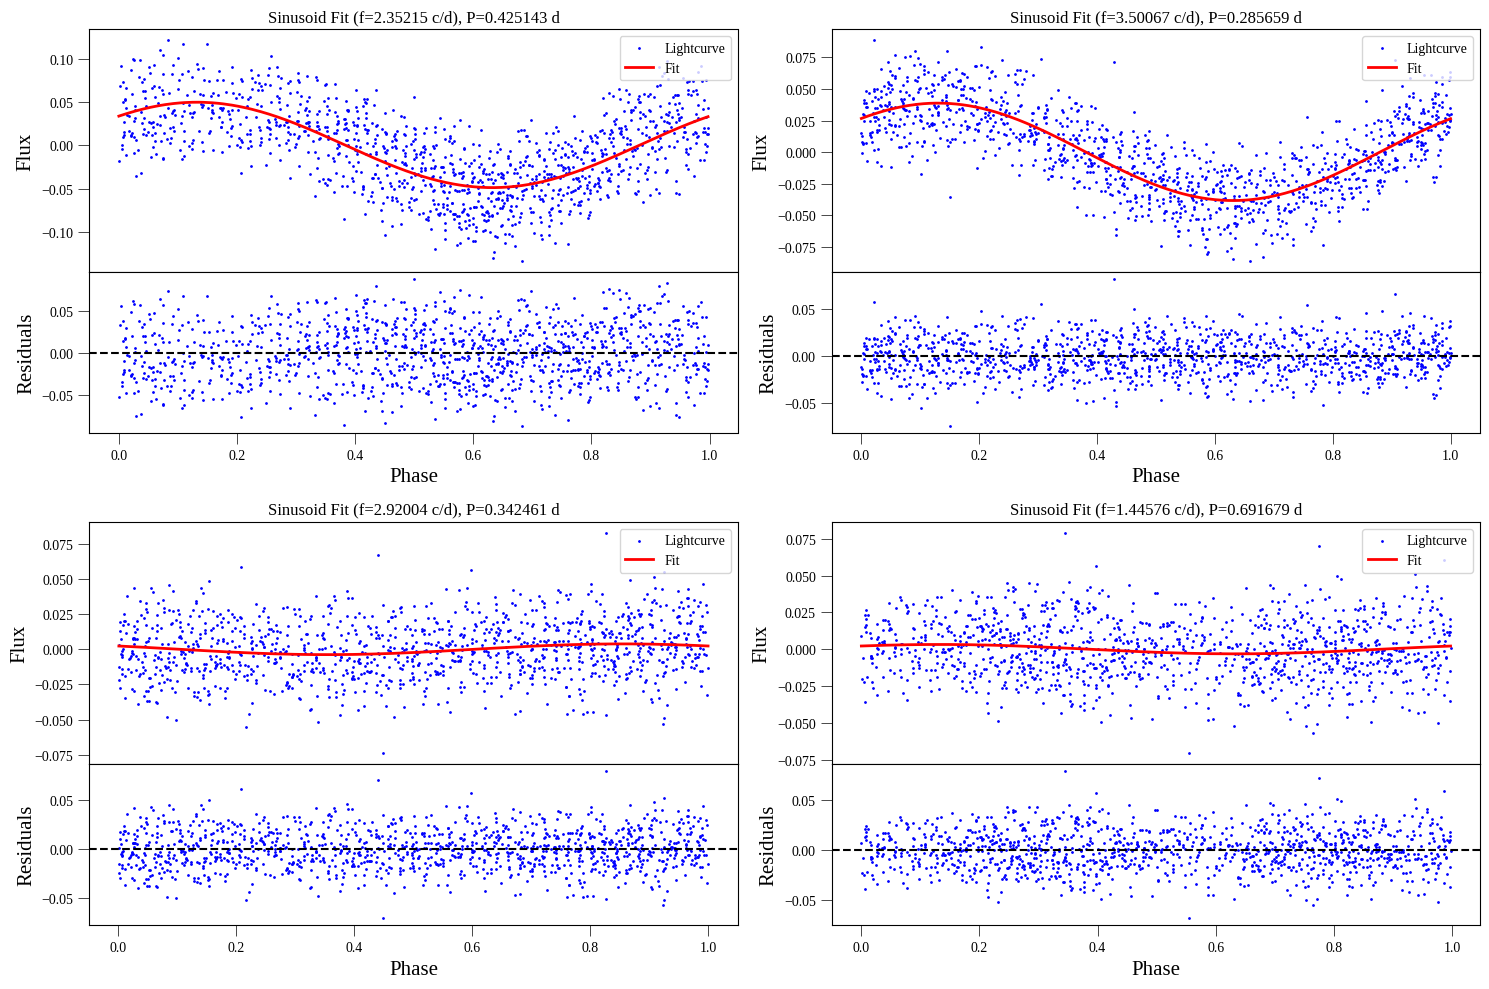
\includegraphics[width=0.9\textwidth]{phase/3_phase_folded.png}
        \caption{Fázově složená světelná křivka pro dataset 3.dat.}
        \label{fig:3_phase_folded}
    \end{figure*}

    \begin{figure*}
        \centering
        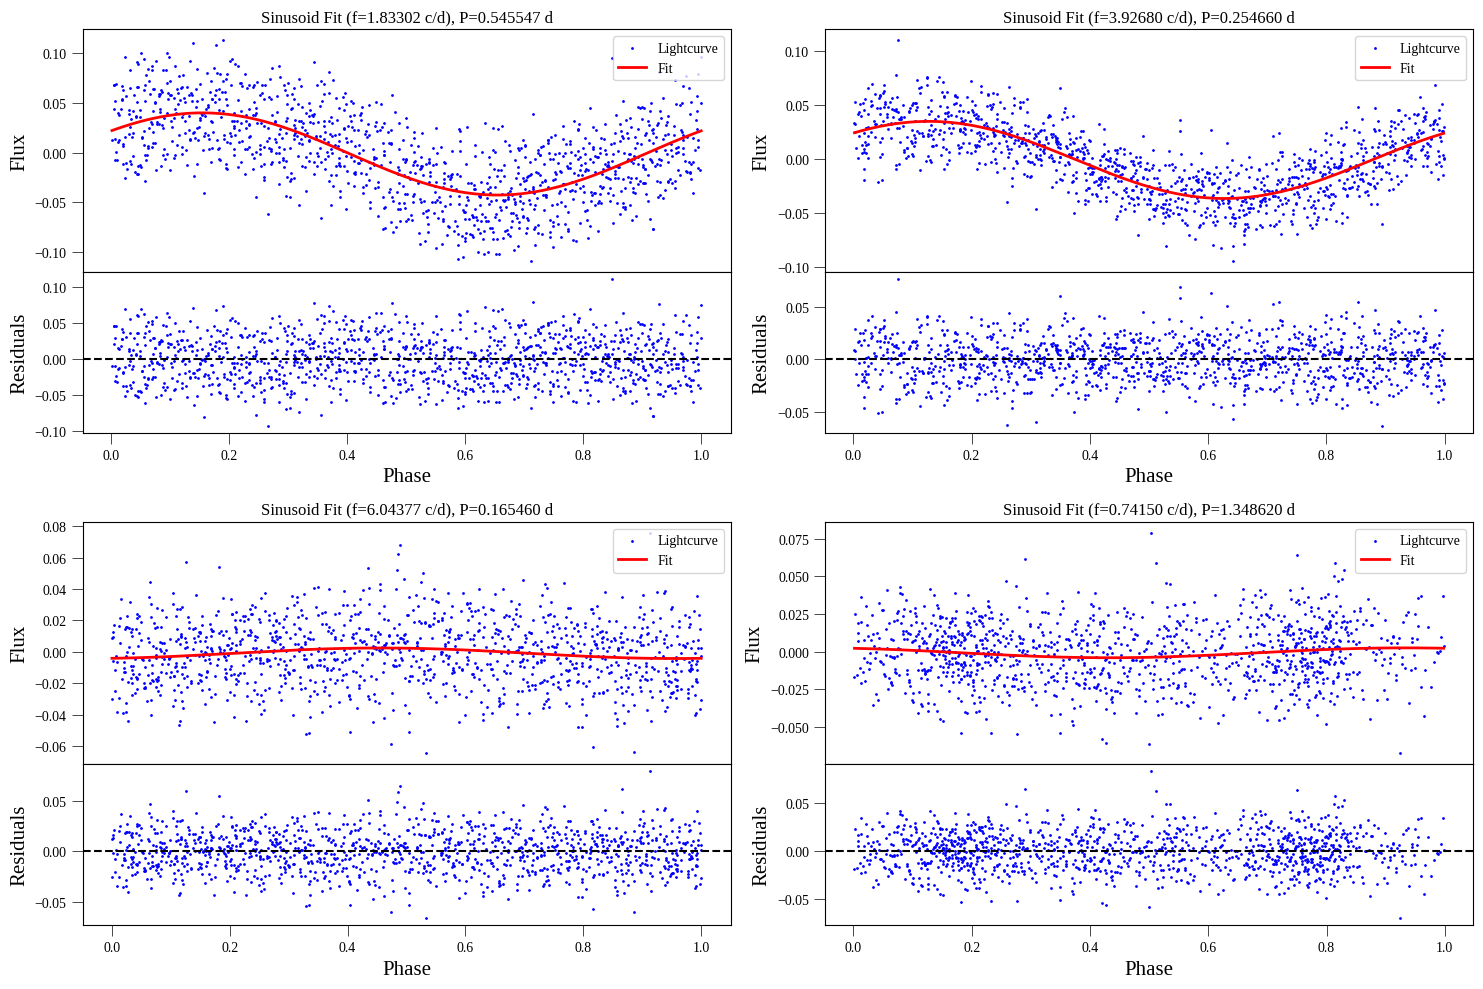
\includegraphics[width=0.9\textwidth]{phase/4_phase_folded.png}
        \caption{Fázově složená světelná křivka pro dataset 4.dat.}
        \label{fig:4_phase_folded}
    \end{figure*}

    \begin{figure*}
        \centering
        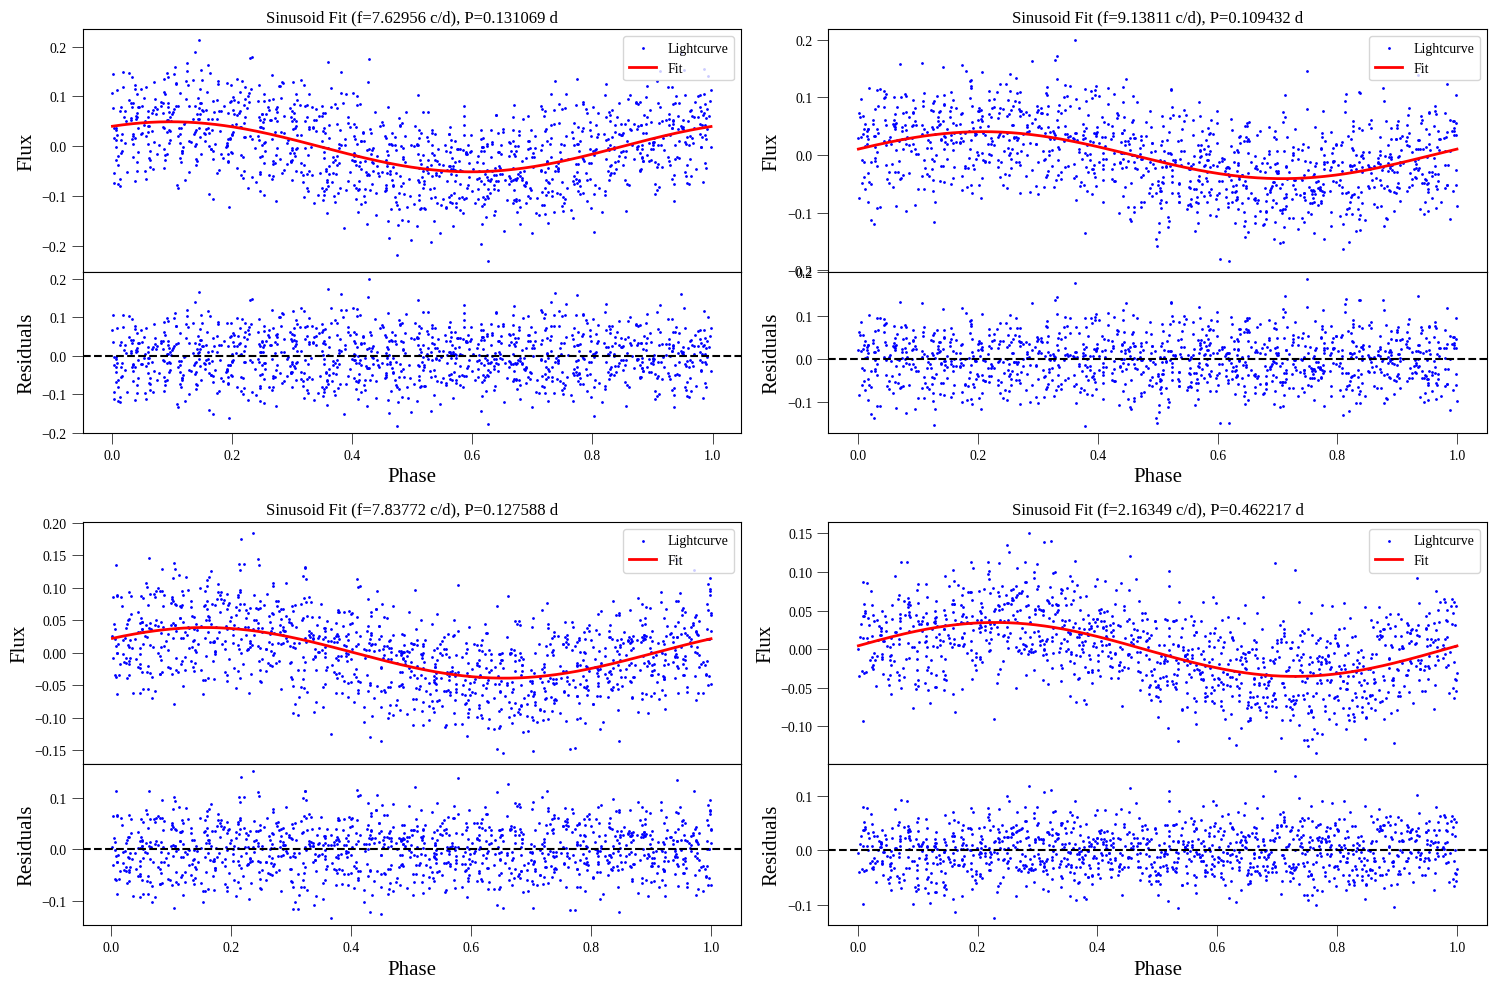
\includegraphics[width=0.9\textwidth]{phase/5_phase_folded.png}
        \caption{Fázově složená světelná křivka pro dataset 5.dat.}
        \label{fig:5_phase_folded}
    \end{figure*}

    \begin{figure*}
        \centering
        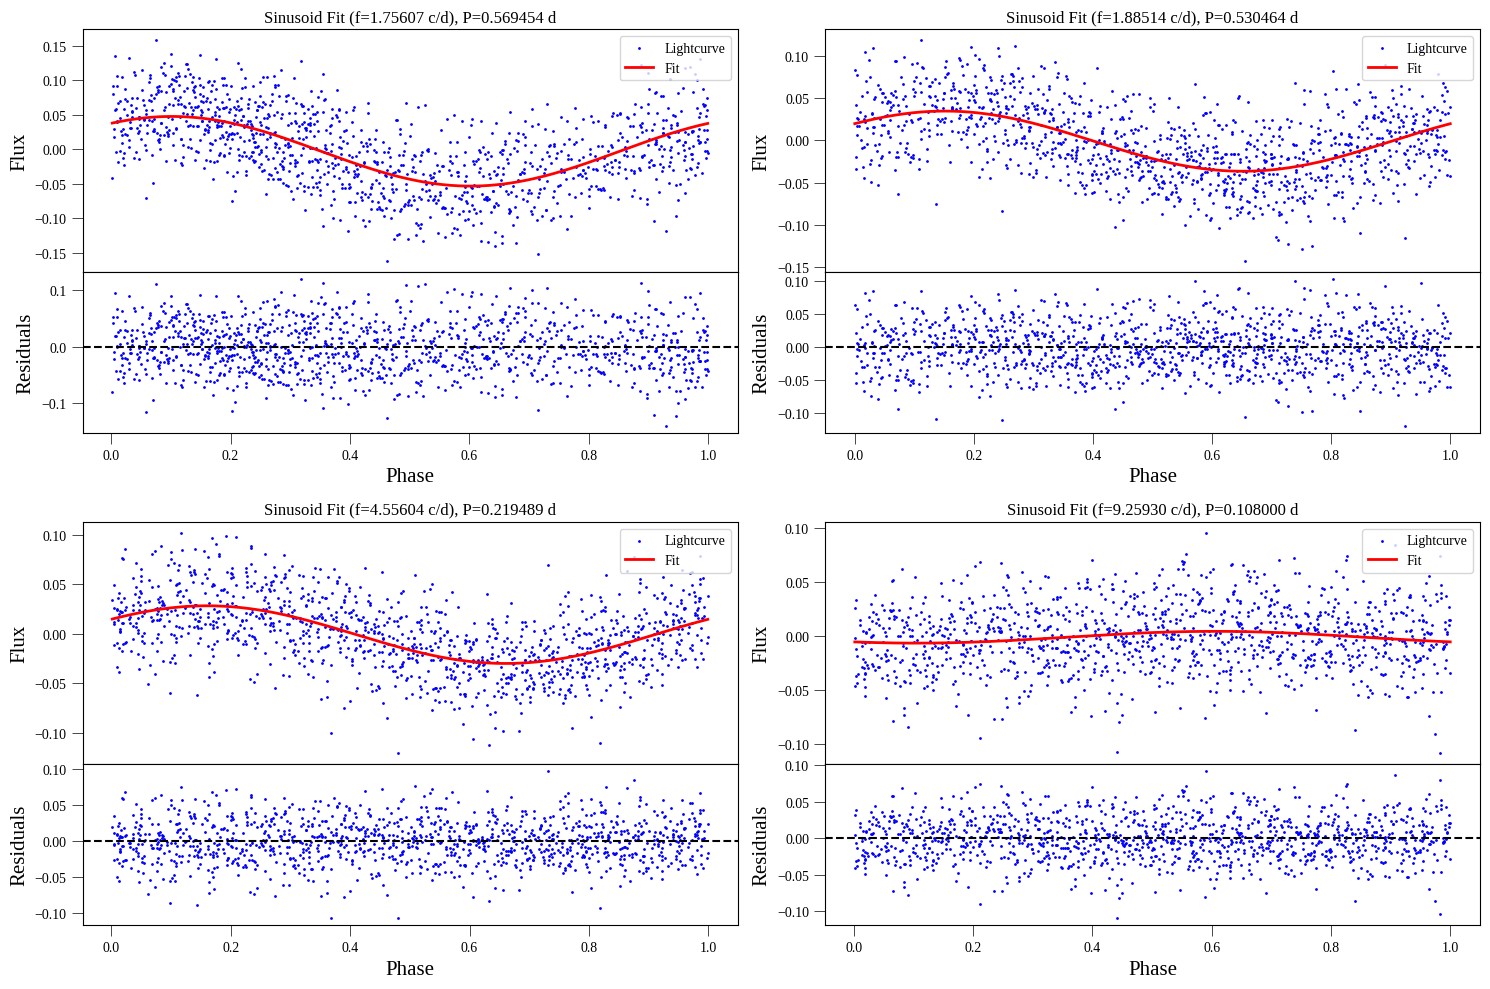
\includegraphics[width=0.9\textwidth]{phase/6_phase_folded.png}
        \caption{Fázově složená světelná křivka pro dataset 6.dat.}
        \label{fig:6_phase_folded}
    \end{figure*}

    %%%% Orginalni fázově složené světelné křivky %%%%
    \begin{figure*}
        \centering
        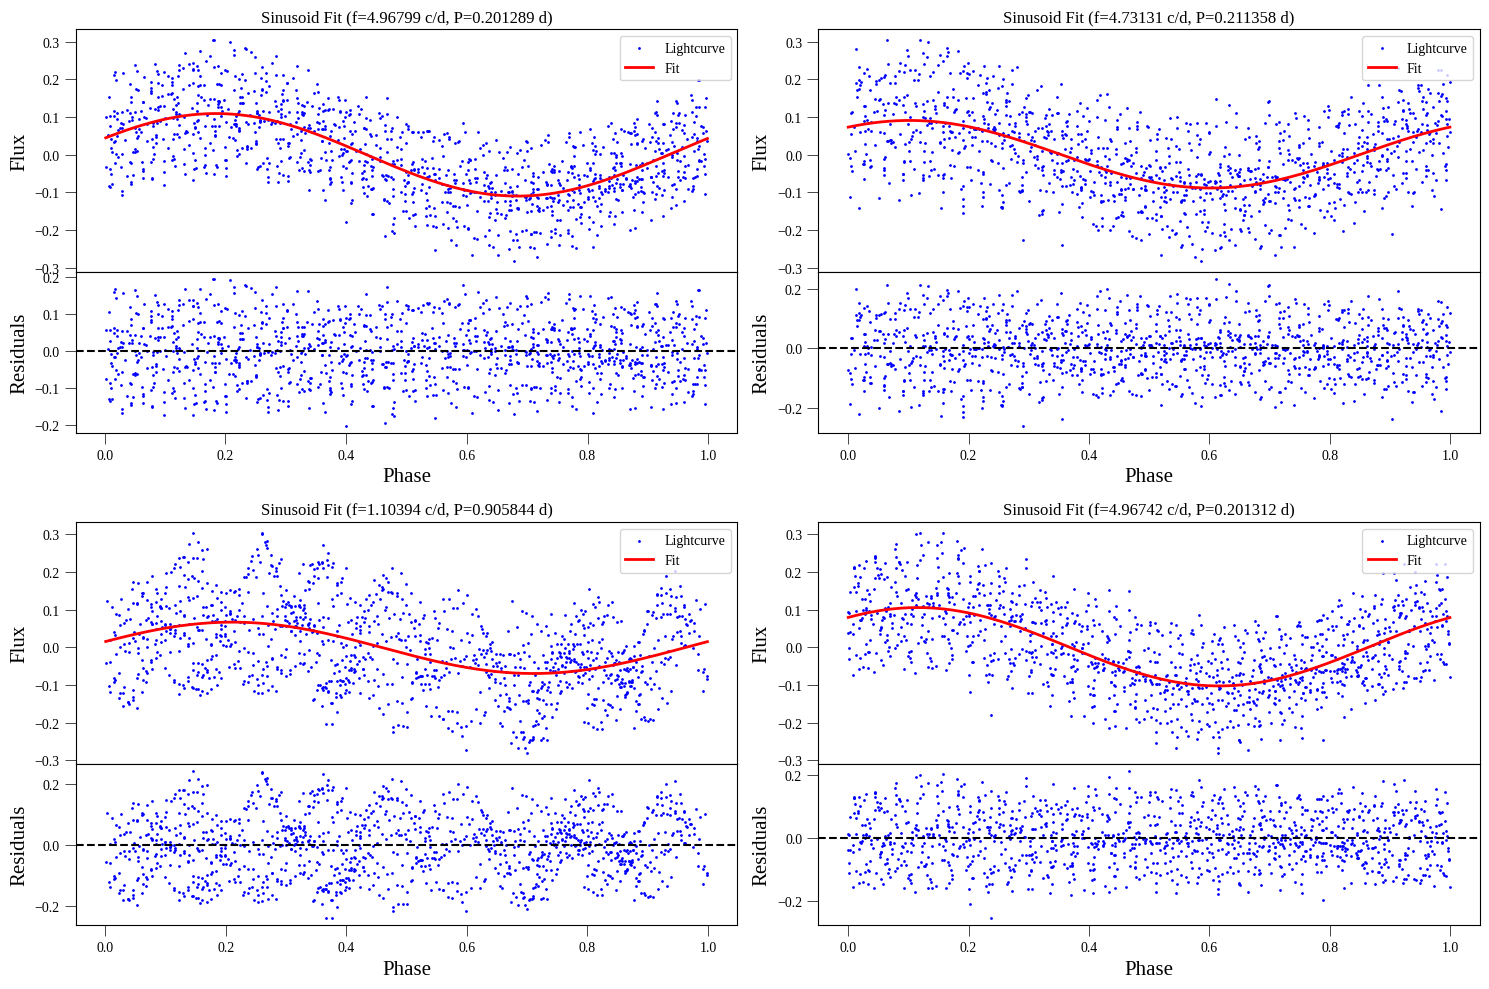
\includegraphics[width=0.9\textwidth]{phase/1_phase_folded_orig.png}
        \caption{Orginalni fázově složená světelná křivka pro dataset 1.dat.}
        \label{fig:1_phase_folded_orig}
    \end{figure*}

    \begin{figure*}
        \centering
        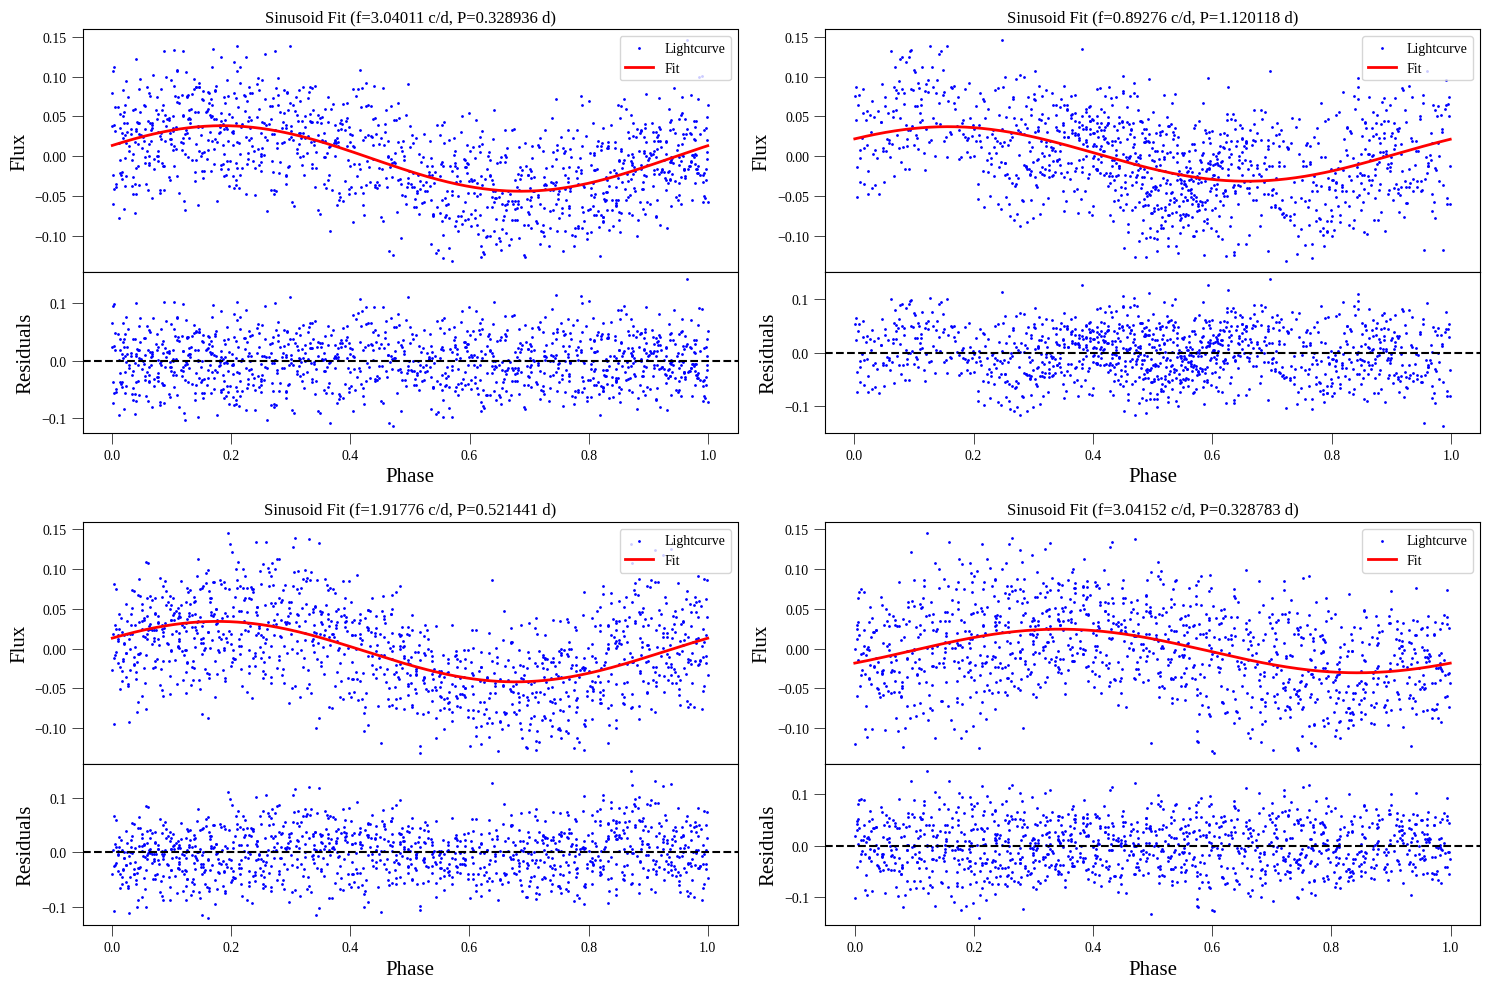
\includegraphics[width=0.9\textwidth]{phase/2_phase_folded_orig.png}
        \caption{Orginalni fázově složená světelná křivka pro dataset 2.dat.}
        \label{fig:2_phase_folded_orig}
    \end{figure*}

    \begin{figure*}
        \centering
        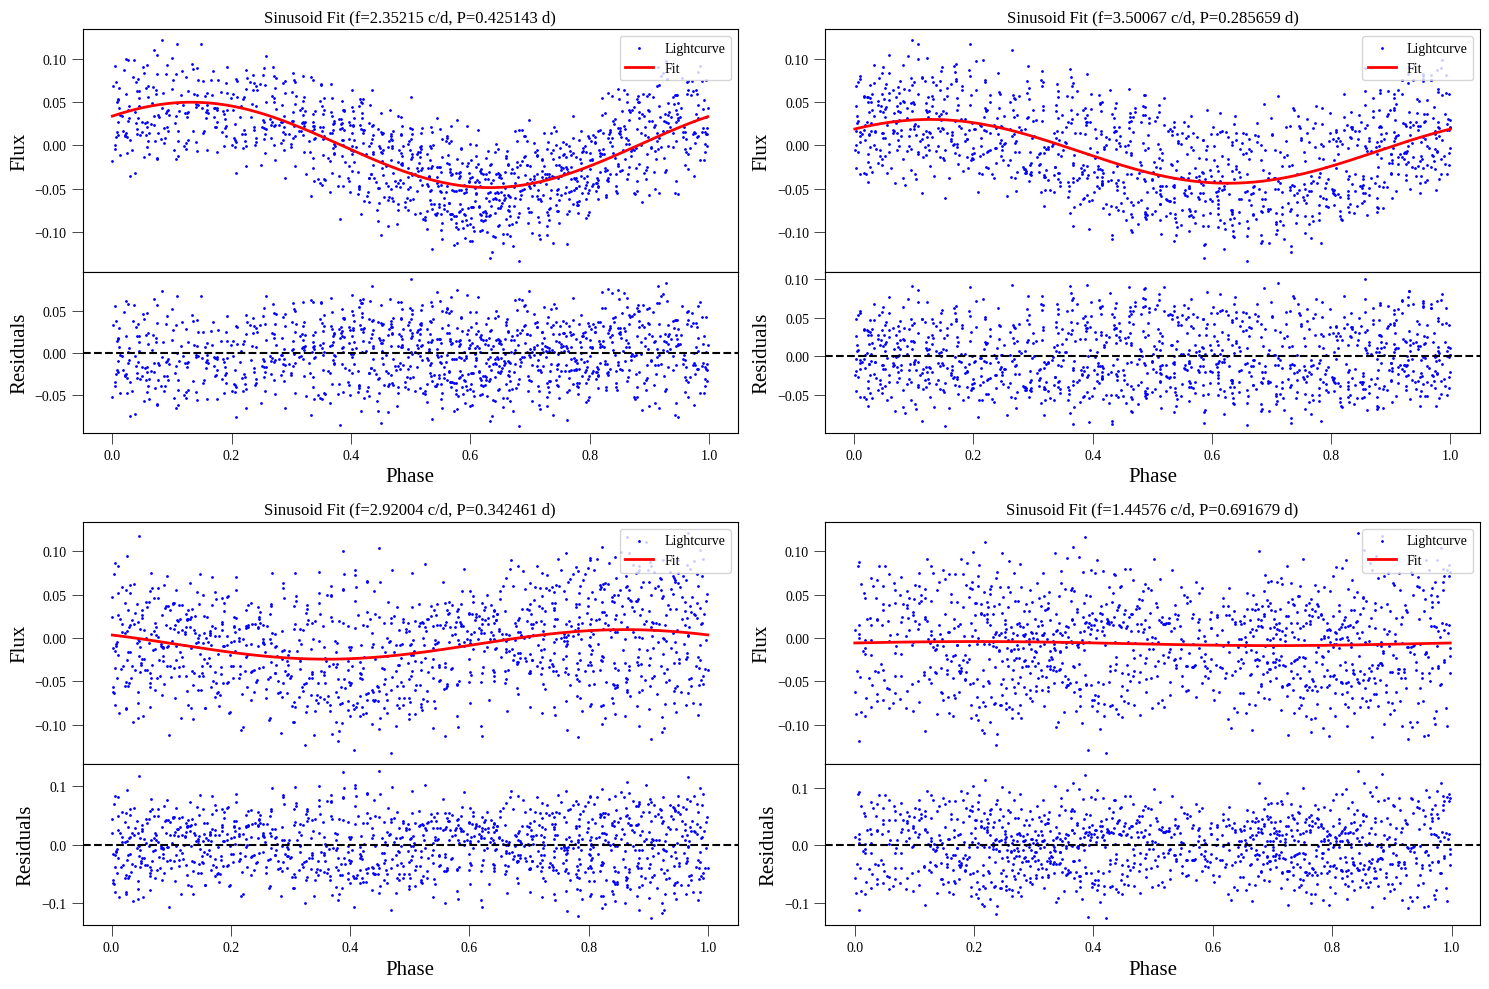
\includegraphics[width=0.9\textwidth]{phase/3_phase_folded_orig.png}
        \caption{Orginalni fázově složená světelná křivka pro dataset 3.dat.}
        \label{fig:3_phase_folded_orig}
    \end{figure*}

    \begin{figure*}
        \centering
        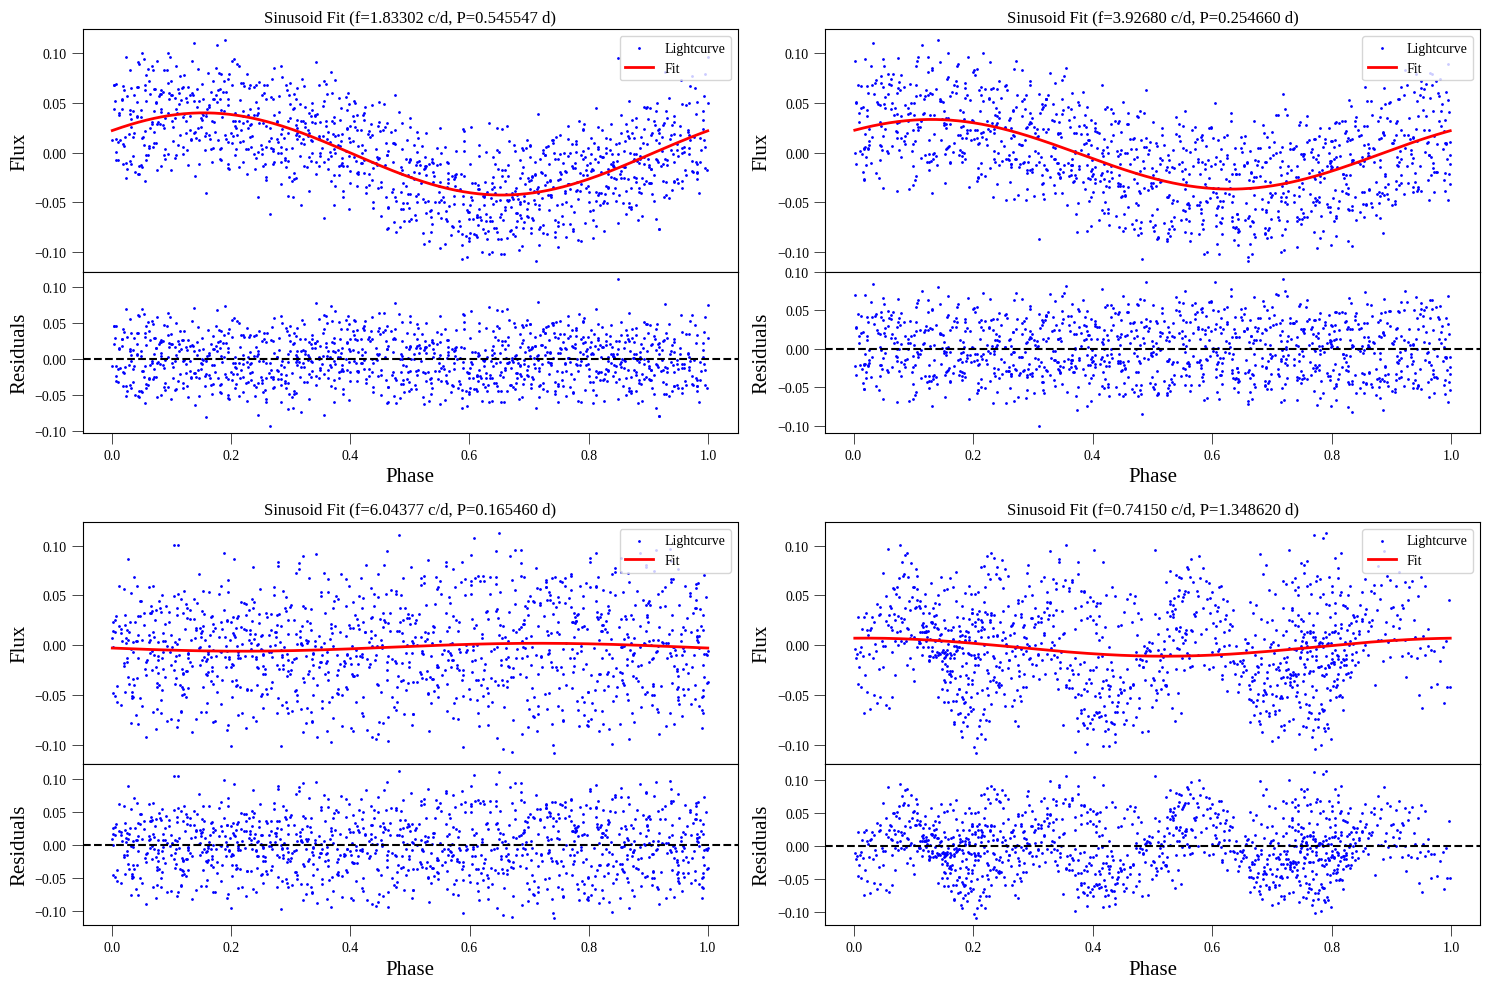
\includegraphics[width=0.9\textwidth]{phase/4_phase_folded_orig.png}
        \caption{Orginalni fázově složená světelná křivka pro dataset 4.dat.}
        \label{fig:4_phase_folded_orig}
    \end{figure*}

    \begin{figure*}
        \centering
        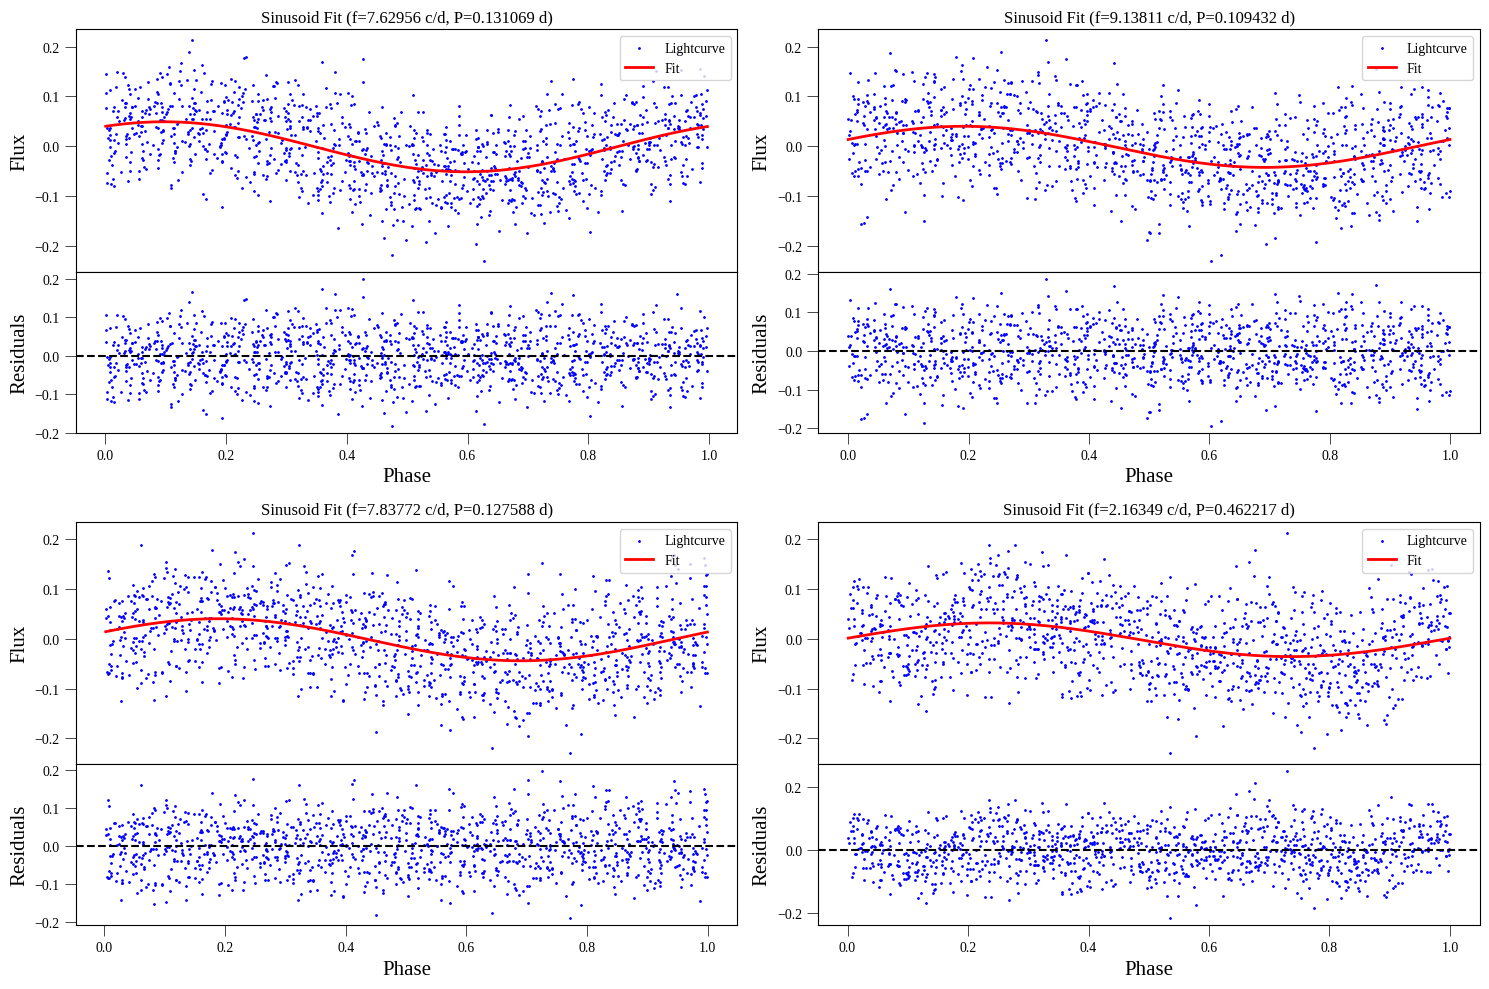
\includegraphics[width=0.9\textwidth]{phase/5_phase_folded_orig.png}
        \caption{Orginalni fázově složená světelná křivka pro dataset 5.dat.}
        \label{fig:5_phase_folded_orig}
    \end{figure*}

    \begin{figure*}
        \centering
        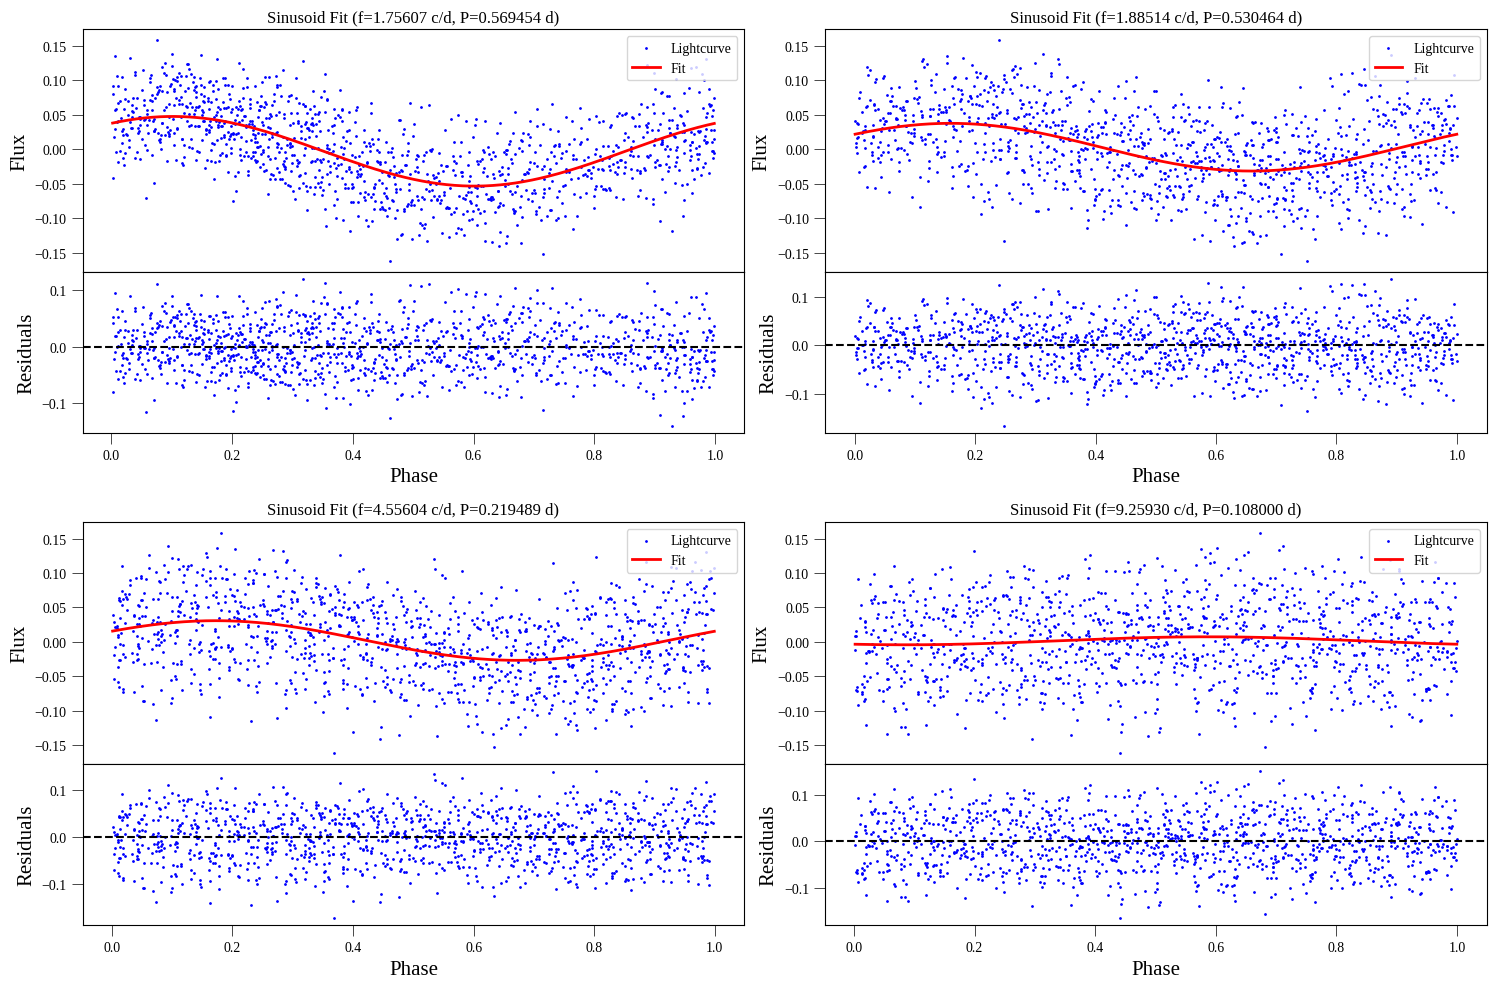
\includegraphics[width=0.9\textwidth]{phase/6_phase_folded_orig.png}
        \caption{Orginalni fázově složená světelná křivka pro dataset 6.dat.}
        \label{fig:6_phase_folded_orig}
    \end{figure*}

    %%%% Kepler-1063 %%%%
    \begin{figure*}
        \centering
        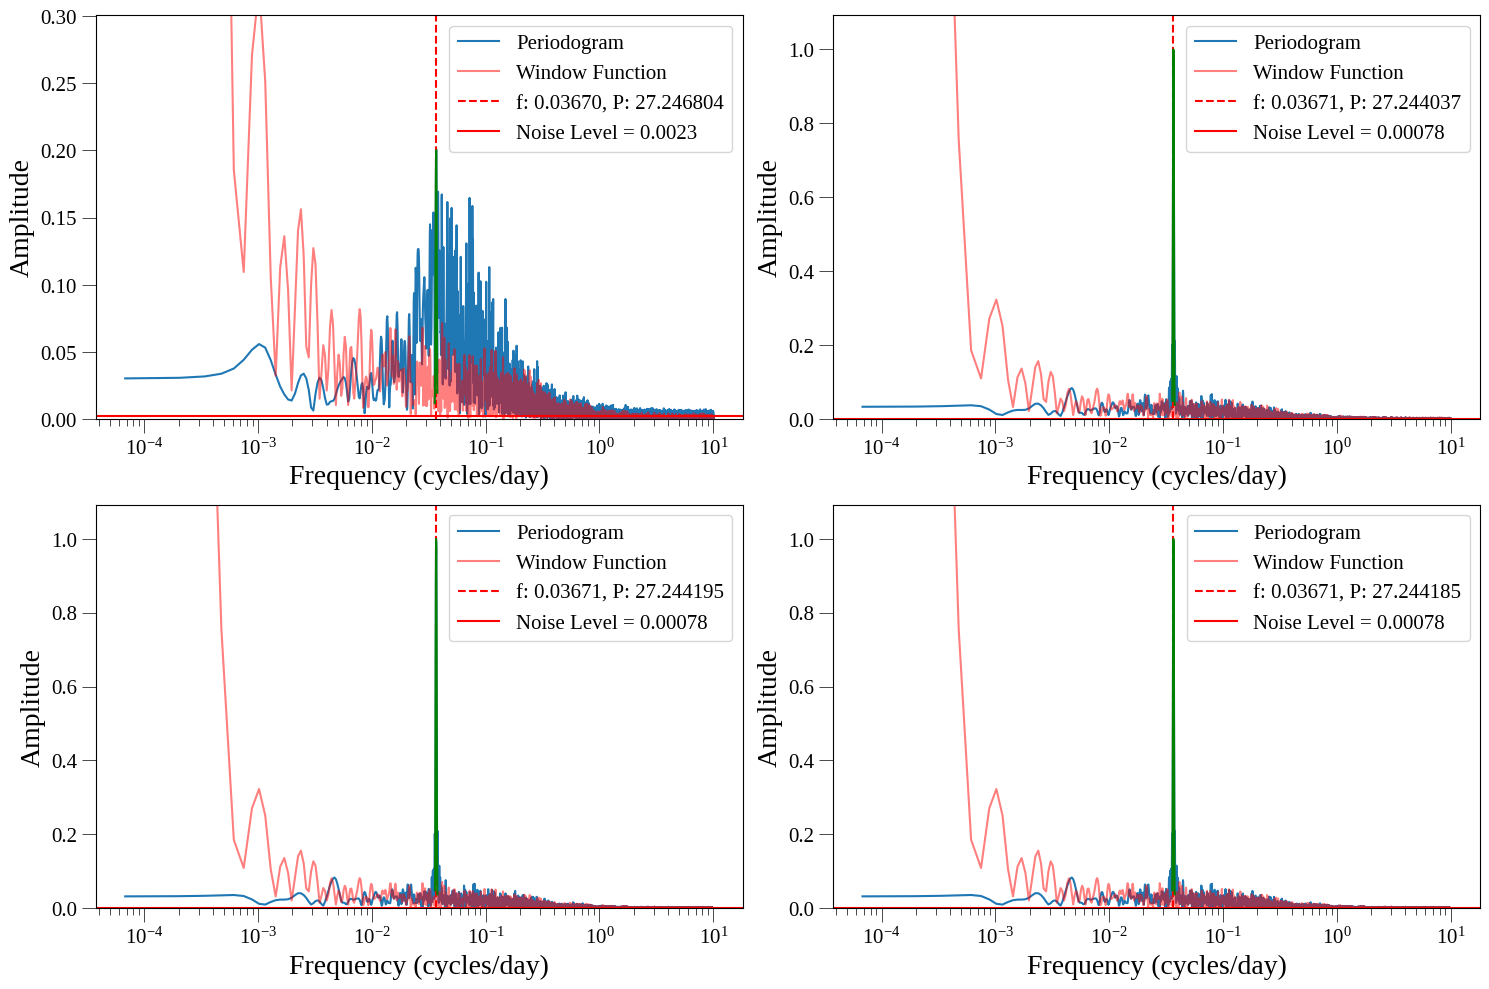
\includegraphics[width=0.9\textwidth]{period/Kepler-1063_per.png}
        \caption{Periodogram pro Kepler-1063.}
        \label{fig:kplr_per}
    \end{figure*}

    \begin{figure*}
        \centering
        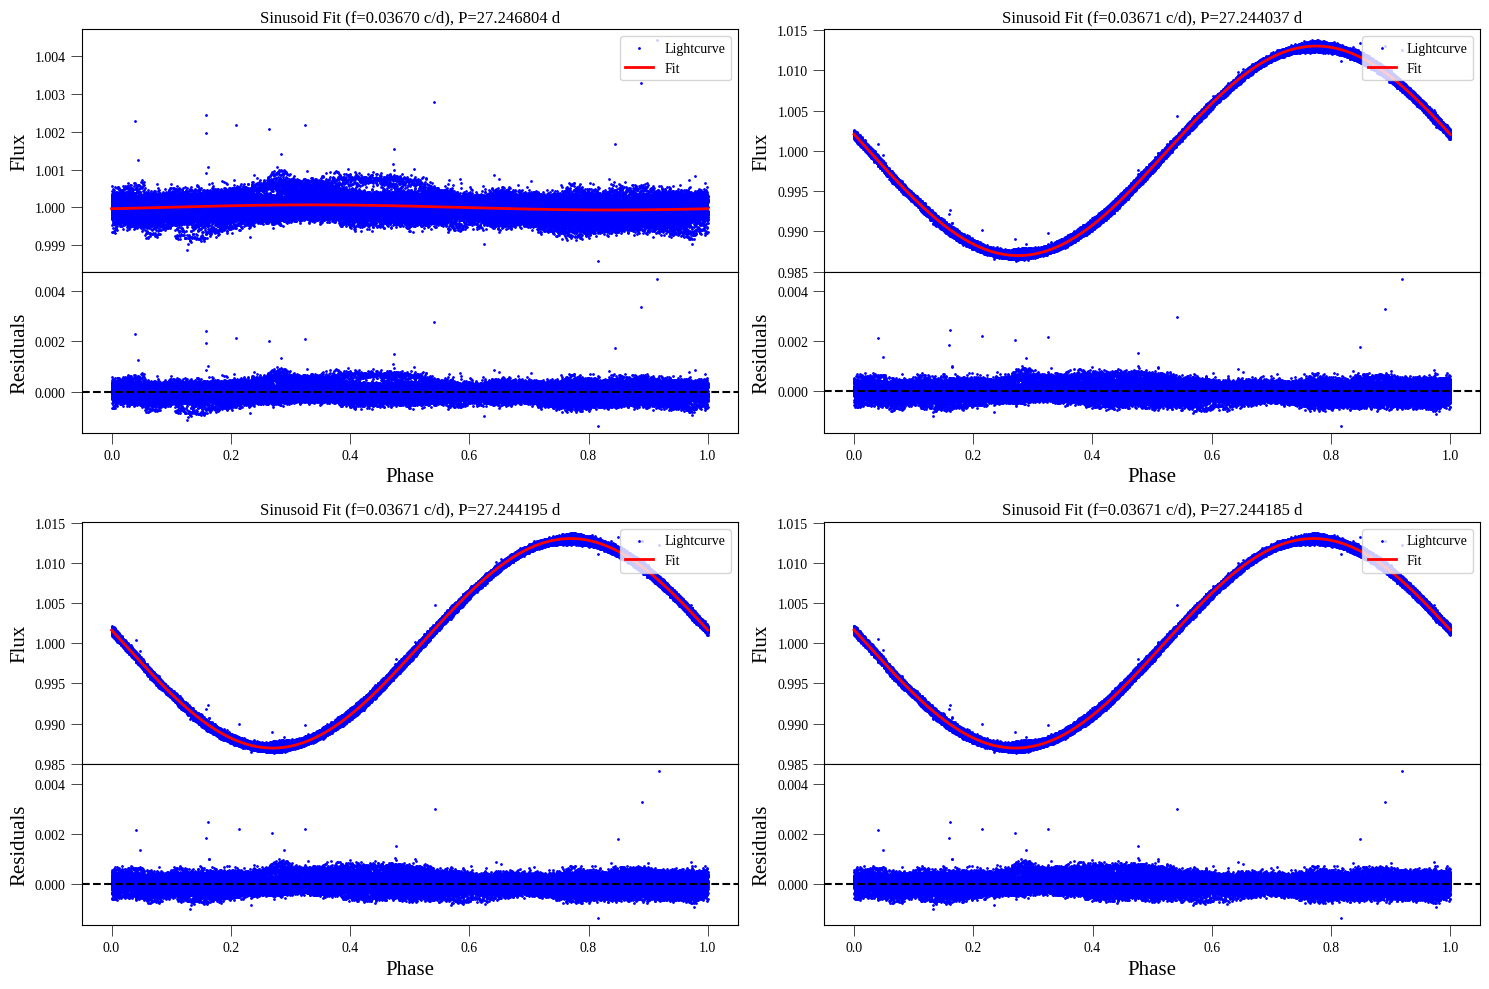
\includegraphics[width=0.9\textwidth]{phase/Kepler-1063_phase_folded.png}
        \caption{Fázově složená světelná křivka pro Kepler-1063.}
        \label{fig:kplr_phase_folded}
    \end{figure*}

    \begin{figure*}
        \centering
        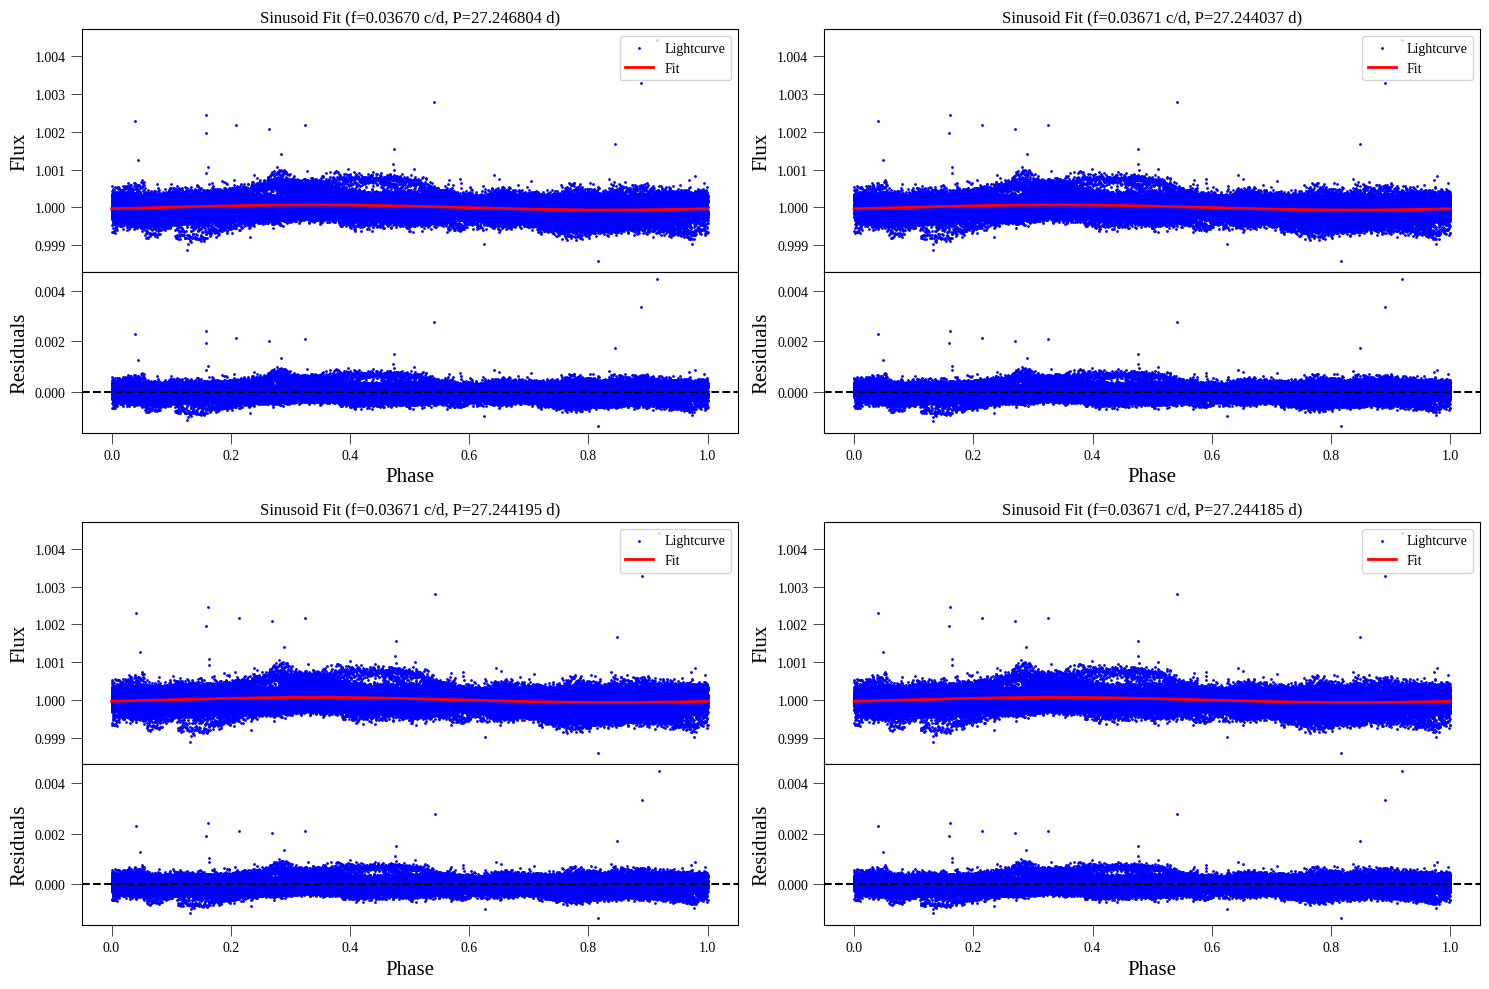
\includegraphics[width=0.9\textwidth]{phase/Kepler-1063_phase_folded_orig.png}
        \caption{Orginalni fázově složená světelná křivka pro Kepler-1063.}
        \label{fig:kplr_phase_folded_orig}
    \end{figure*}

    \begin{figure*}
        \centering
        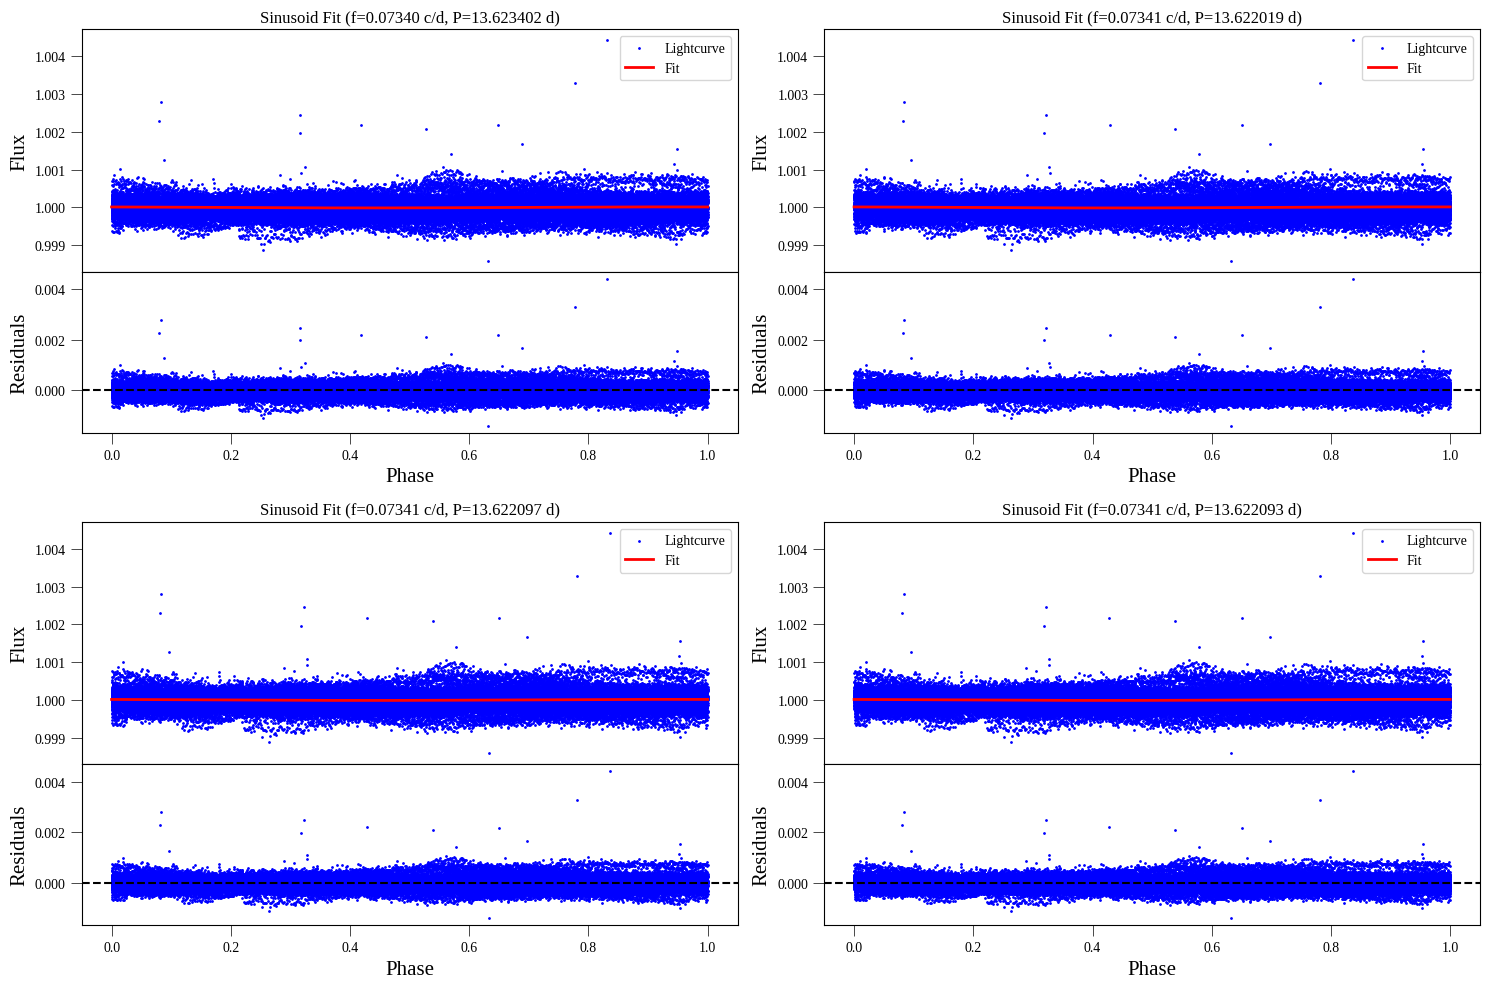
\includegraphics[width=0.9\textwidth]{phase/Kepler-1063_phase_folded_orig_teor.png}
        \caption{Orginalni fázově složená světelná křivka pro Kepler-1063 s poloviční periodou.}
        \label{fig:Kepler-1063_phase_folded_orig_teor}
    \end{figure*}

\end{document}